\documentclass[a4paper, 11pt, openany]{report}

\usepackage{ensa-a} %%%%Important to use functionalities used in the vid. 
\usepackage{float}


\begin{document}


\pagedegarde{ENSA4/GI/23-24}{d'annee}{Abdelhak Mekaoui}{Adil Abbadi}{Genie Informatique}{Conception, Developpement et Deploiement d'un Chatbot Inte lligent et d'une Plate forme E-Learning}{M. A EL YOUSFI}{M. H Elkina}{images/code.png}{0.5}{M. H AKSASSE}{M. M ELYAAKOUBI}{03/06/2024}
\Newpage


\chaptertoc{Dedicace}

\lettrine[nindent=0em, slope=-.5em]{\color{Eblue}N}{ous} souhaitons exprimer notre profonde gratitude à toutes les personnes qui ont contribue à notre parcours et à la realisation de ce projet. En particulier, nous tenons à remercier nos chers parents, pour leur soutien indefectible, leurs sacrifices et leur amour inconditionnel. Ils ont ete les piliers de notre education et les premiers architectes de nos rêves. À nos frères et sœurs, pour leur soutien constant et leur presence reconfortante à chaque etape de notre vie. Nous leur dedions ce travail en signe d'affection et de reconnaissance pour leur precieuse contribution à notre epanouissement.

\ \\
\lettrine[nindent=0em, slope=-.5em]{\color{Eblue}À}{ notre} famille et à nos amis, pour leur soutien infaillible, leur encouragement et leur comprehension tout au long de notre parcours. Leur presence à nos côtes a ete une source de force et de motivation.

\ \\
\lettrine[nindent=0em, slope=-.5em]{\color{Eblue}À}{ nos} encadrants et à nos respectables professeurs, nous exprimons notre gratitude pour leur expertise, leurs conseils avises et leur accompagnement precieux. Leur enseignement et leur soutien ont ete determinants dans notre formation et dans la reussite de ce projet.

\ \\
\lettrine[nindent=0em, slope=-.5em]{\color{Eblue}E}{nfin}, à toutes les personnes qui nous ont apporte du bonheur et de la joie dans notre vie, qui ont ete les jardiniers de nos âmes, nous vous dedions egalement ce travail. Vos sourires, vos encouragements et votre bienveillance ont enrichi notre parcours et nous ont inspires à donner le meilleur de nous-mêmes.

\ \\
\lettrine[nindent=0em, slope=-.5em]{\color{Eblue}P}{uissent} ces mots temoigner de notre reconnaissance eternelle et de notre profond respect envers tous ceux qui ont contribue à notre reussite.



\newpage


\chaptertoc{Remerciment}

\lettrine[nindent=0em, slope=-.5em]{\color{Eblue}N}{ous} souhaitons tout d'abord exprimer notre profonde gratitude à notre ecole, \textbf{ENSA Agadir}, pour nous avoir offert ces opportunites precieuses et pour leur soutien indefectible tout au long de notre parcours academique. L'ENSA Agadir a joue un rôle crucial en nous offrant un environnement d'apprentissage enrichissant et en nous preparant à relever les defis professionnels.

\ \\

\lettrine[nindent=0em, slope=-.5em]{\color{Eblue}U}{n} remerciement tout particulier à \textbf{M. EL YOUSFI Abderrahmane}, notre encadrant à l'ecole, dont la guidance perspicace et les conseils avises ont ete des elements cles dans la reussite de notre projet. Votre engagement, votre patience et votre volonte de partager vos connaissances ont profondement enrichi notre experience. Merci d'avoir ete une source constante de motivation et de soutien. Unifies tous, chaque jour etait une aventure passionnante. Merci d'avoir cree un environnement de travail stimulant où nous avons pu grandir et nous epanouir professionnellement.

\ \\

\lettrine[nindent=0em, slope=-.5em]{\color{Eblue}N}{n}ous tenons aussi à remercier tous les membres du jury \textbf{M. H AKSASSE} et \textbf{M. M ELYAAKOUBI} qui nous ont fait l’honneur d’accepter de juger notre travail.

\ \\

\lettrine[nindent=0em, slope=-.5em]{\color{Eblue}N}{ous} tenons à exprimer notre profonde gratitude à toute l'equipe du \textbf{Centre Code 212}, en particulier à \textbf{Hamza el Kina}, le responsable du centre, pour votre devouement et votre soutien constants. Travailler avec vous a ete une opportunite precieuse qui nous a permis d'apprendre enormement grâce à votre expertise. Unis par notre engagement envers l'excellence, nous sommes reconnaissants d'avoir fait partie d'une equipe aussi dynamique et talentueuse que la vôtre. Votre passion pour l'innovation nous a inspires à repousser nos limites et à atteindre de nouveaux sommets. collaborer avec vous a ete une experience enrichissante, et votre professionnalisme ainsi que votre soutien inestimable ont joue un rôle essentiel dans notre developpement professionnel. Merci d'avoir ete des mentors exceptionnels. Kudos à toute l'equipe du \textbf{Centre Code 212} pour votre esprit d'equipe et votre determination à surmonter les defis. Votre creativite et votre ingeniosite ont ete une source d'inspiration constante.

\ \\







\Newpage

\chaptertoc{Resume}

\lettrine[nindent=0em, slope=-.5em]{\color{Eblue}L}{e} present document est une synthèse de notre projet de fin d’annee realise au sein de l'entreprise \textbf{Code212}. Durant ce stage, nous avons eu la chance de travailler sur un projet informatique visant à integrer un chatbot intelligent dans la plateforme e-learning de \textbf{Code212}.

\ \\

\lettrine[nindent=0em, slope=-.5em]{\color{Eblue}L}{e} projet consiste à creer et à integrer un chatbot AI dans une application web dediee à la formation en ligne et la gestion des cours et certificats pour les etudiants. Les utilisateurs de la plateforme incluent des etudiants, des gestionnaires et des administrateurs. Les etudiants pourront interagir avec le chatbot pour obtenir des informations sur les cours, s'inscrire à des evenements et examens de certification, et recevoir de l'aide personnalisee. Les gestionnaires auront la possibilite de creer, modifier et supprimer des cours, evenements et certificats. Les administrateurs seront charges de gerer les utilisateurs et d'assurer le bon fonctionnement de la plateforme.

\ \\

\lettrine[nindent=0em, slope=-.5em]{\color{Eblue}L}{e} chatbot AI est conçu pour ameliorer l'efficacite et l'accessibilite des services de formation en ligne, offrant une assistance immediate et personnalisee aux utilisateurs. Grâce à cette integration, les etudiants beneficieront d'une interface interactive et intuitive, facilitant leur parcours d'apprentissage.

\ \\

\lettrine[nindent=0em, slope=-.5em]{\color{Eblue}A}{fin} de gerer au mieux ce projet, nous avons opte pour la methode \textbf{SCRUM} et divise les differents modules en sprints. Un sprint de preparation a ete initie pour effectuer une analyse fonctionnelle globale et construire un modèle de base pour les sprints suivants. Après avoir termine le sprint de preparation, nous avons execute les autres sprints, chacun etant dedie à la conception detaillee d’un module de l’application, suivi par l'elaboration de ses maquettes et enfin sa realisation.

\ \\

\lettrine[nindent=0em, slope=-.5em]{\color{Eblue}E}{n} resume, le projet vise à integrer un chatbot AI dans une plateforme e-learning, offrant une experience d'apprentissage amelioree pour les etudiants et une gestion efficace des cours et evenements pour les gestionnaires et administrateurs. Cette integration assure une interaction fluide et securisee, tout en augmentant l'accessibilite et l'efficacite des services educatifs en ligne de \textbf{Code212}.

\newpage
\chapter*{Abstract}

\lettrine[nindent=0em, slope=-.5em]{\color{Eblue}T}{his} document is a summary of our end-of-year project conducted within the company \textbf{Code212}. During this internship, we had the opportunity to work on an IT project aimed at integrating an intelligent chatbot into the \textbf{Code212} e-learning platform.

\ \\

\lettrine[nindent=0em, slope=-.5em]{\color{Eblue}T}{he} project involves creating and integrating an AI chatbot into a web application dedicated to online training and managing courses and certificates for students. The platform users include students, managers, and administrators. Students will be able to interact with the chatbot to get information about courses, register for events and certification exams, and receive personalized assistance. Managers will have the ability to create, modify, and delete courses, events, and certificates. Administrators will be responsible for managing users and ensuring the smooth operation of the platform.

\ \\

\lettrine[nindent=0em, slope=-.5em]{\color{Eblue}T}{he} AI chatbot is designed to improve the efficiency and accessibility of online training services, providing immediate and personalized assistance to users. With this integration, students will benefit from an interactive and intuitive interface, facilitating their learning journey.

\ \\

\lettrine[nindent=0em, slope=-.5em]{\color{Eblue}I}{n} order to manage this project effectively, we opted for the \textbf{SCRUM} methodology and divided the different modules into sprints. An initial sprint was initiated to perform a comprehensive functional analysis and build a baseline model for the following sprints. After completing the initial sprint, we executed the other sprints, each dedicated to the detailed design of a module of the application, followed by the development of its prototypes, and finally its implementation.

\ \\

\lettrine[nindent=0em, slope=-.5em]{\color{Eblue}I}{n} summary, the project aims to integrate an AI chatbot into an e-learning platform, offering an enhanced learning experience for students and efficient management of courses and events for managers and administrators. This integration ensures smooth and secure interaction while increasing the accessibility and efficiency of \textbf{Code212}'s online educational services.
\newpage

\tableofcontents
\listoffigures
\listoftables



\newpage
\chapter*{Abreviations}
\begin{tabular}{ll}
\textbf{Abreviation} & \textbf{Signification} \\
\hline
LLM & Large Language Model \\
HTML & HyperText Markup Language \\
FASTAPI & Fast API framework \\
API & Application Programming Interface \\
AI & Artificial Intelligence \\
ML & Machine Learning \\
NLP & Natural Language Processing \\
SQL & Structured Query Language \\
JSON & JavaScript Object Notation \\
REST & Representational State Transfer \\
RAG & Retrieval-Augmented Generation \\
HTTP & Hypertext Transfer Protocol \\
HTTPS & Hypertext Transfer Protocol Secure \\
XML & Extensible Markup Language \\
CSV & Comma-Separated Values \\
UI & User Interface \\
UX & User Experience \\
CRUD & Create, Read, Update, Delete \\
SaaS & Software as a Service \\
PaaS & Platform as a Service \\
IaaS & Infrastructure as a Service \\
SDK & Software Development Kit \\
IDE & Integrated Development Environment \\
CI/CD & Continuous Integration/Continuous Deployment \\
OOP & Object-Oriented Programming \\
JSON & JavaScript Object Notation \\
JWT & JSON Web Token \\
DOM & Document Object Model \\
TDD & Test-Driven Development \\
ORM & Object-Relational Mapping \\
CLI & Command Line Interface \\
GUI & Graphical User Interface \\
ROI & Return on Investment \\
QA & Quality Assurance \\
\end{tabular}


\chaptertoc{Introduction generale}

\lettrine[nindent=0em, slope=-.5em]{\color{Eblue}A}{u} cours des deux dernières decennies, les avancees sans precedent dans le domaine des technologies de l'information ont engendre une veritable revolution, bouleversant profondement notre mode de vie et notre façon de travailler. Cependant, ce dynamisme technologique rapide n'est pas sans consequences. Il pose des defis sociaux, economiques et ethiques qui necessitent une reflexion approfondie et des adaptations constantes. Neanmoins, il est indeniable que les progrès technologiques ont ameliore notre qualite de vie de manière inimaginable, facilitant les tâches quotidiennes, stimulant la creativite, et ouvrant des perspectives sans limites.
\\

La gestion de la formation et de l'assistance technique represente toujours un defi considerable pour les centres de formation, surtout sans l’outil informatique adequat. La tâche devient alors plus complexe et coûteuse en raison des pertes de ressources et de temps liees à une gestion inefficace. L’informatique a prouve son importance en offrant des solutions efficaces pour la gestion des processus pedagogiques, de l’assistance technique, et des services divers, apportant un gain de temps et une simplification des tâches.
\\
L'introduction des chatbots intelligents, alimentes par l'intelligence artificielle (IA), apporte des benefices multiples dans divers domaines, y compris l'education et la formation. Ces assistants virtuels automatises peuvent interagir avec les utilisateurs de manière conversationnelle, offrant ainsi une assistance instantanee et personnalisee. Les applications des chatbots en general incluent :
\begin{itemize}
    \item \textbf{Assistance Instantanee} : Les etudiants beneficient d'une aide immediate pour leurs questions frequentes, ce qui facilite un apprentissage autonome et renforce le processus educatif.
    \item \textbf{Amelioration de l'Employabilite} : En fournissant des outils pratiques et interactifs pour la formation, Code212 prepare mieux ses etudiants à integrer le marche du travail numerique.
    \item \textbf{Optimisation des Ressources} : Le chatbot aide à une utilisation plus efficace des ressources pedagogiques disponibles, maximisant ainsi l'efficacite des etudes des apprenants.
    \item \textbf{Support Moral} : En offrant un soutien empathique et motivant, le chatbot contribue à maintenir la perseverance et l'engagement des etudiants.
\end{itemize}
\ \\

C’est dans ce contexte que notre projet de fin d’annee a vu le jour, au sein du centre Code212 de l’Universite Ibn Zohr. Le projet consiste à elaborer un assistant chatbot intelligent et à l'integrer dans une plateforme e-learning pour le centre Code212. Ces outils visent à ameliorer l’efficacite de la formation et de l'assistance technique, en permettant une interaction centralisee et accessible via Internet.
\\

Pour repondre au besoin, nous avons opte pour la methode Scrum pour notre projet. Cette methode favorise une flexibilite et une adaptation continues aux exigences changeantes du client. Nous avons utilise des outils et frameworks d'IA tels que Hugging Face, Transformers, LLaMA2 et LangChain pour renforcer les capacites de notre chatbot intelligent. En complement, nous avons utilise le framework Spring Boot, Next.js et FastAPI, completes par Tailwind CSS pour la conception de l’interface utilisateur. Cette combinaison de technologies nous a permis de developper des solutions performantes et efficaces. 
\\

Le present document comporte cinq chapitres : le premier, contexte general du projet, presente l’entreprise d’accueil et le projet ; le deuxième, analyse et conception, decrit les besoins, le cahier des charges et le prototypage et modelise le projet sous forme de diagrammes de cas d’utilisation, de sequence et de classes; le troisième, etude technique, contient l'architecture et le technologies utilisees ; le quatrième, dedie au realisation et mise en oeuvre lors du developpement de cette application ; et enfin, le cinquième chapitre, conclusion generale, devoile les principales interfaces realisees.
\\

Ce projet nous a permis de demontrer l'importance et l’efficacite des technologies de l'information pour la gestion des services de formation et d’assistance, tout en garantissant une satisfaction totale de notre client grâce à une solution securisee et durable.







\chapter{Contexte general du projet :}
\section{Presentation du centre :}
Le Code 212 est un centre de formation et de certification dans les metiers du digital, lance dans le cadre du Plan d'Acceleration de la Croissance et de la Transformation de l'economie (PACTE) ESRI-2030 au Maroc. Ce programme vise à repondre aux enjeux actuels et futurs lies à l'emergence des technologies numeriques en offrant des filières specifiques et des formations certifiantes. L'objectif est de renforcer les competences et les qualifications dans le secteur numerique, contribuant ainsi à l'atteinte des objectifs de developpement du pays, notamment celui de faire passer la part du secteur numerique à 5% du PIB d'ici 2035.

Le principal objectif du Centre Code 212 est de former une nouvelle generation de professionnels qualifies dans le domaine du numerique afin de repondre aux besoins croissants du marche de l'emploi dans ce secteur en plein essor. En offrant des formations specialisees et des certifications reconnues, le centre vise à fournir aux apprenants les competences et les connaissances necessaires pour reussir dans des domaines tels que le developpement web, la cybersecurite, l'analyse de donnees, le marketing digital et bien d'autres. En outre, le centre s'engage à promouvoir l'innovation et l'entrepreneuriat en encourageant les initiatives creatives et en offrant un environnement propice à l'emergence de projets novateurs dans le domaine du digital.

\subsection{Fiche du centre Code 212}

\begin{tabular}{|l|l|}
\hline
\textbf{Nom du Centre} & Code 212 \\
\hline
\textbf{Domaine d'Activite} & Formation et certification dans les metiers du digital \\
\hline
\textbf{Programme} & Plan d'Acceleration de la Croissance et de la Transformation de l'economie (PACTE) ESRI-2030 \\
\hline
\textbf{Localisation} & Maroc \\
\hline
\textbf{Objectif} & Renforcer les competences et les qualifications dans le secteur numerique \\
\hline
\textbf{Contributions} & Atteindre 5\% du PIB du secteur numerique d'ici 2035 \\
\hline
\textbf{Domaines de Formation} & 
\begin{tabular}{@{}l@{}}
- Developpement web \\
- Cybersecurite \\
- Analyse de donnees \\
- Marketing digital \\
- et bien d'autres
\end{tabular} \\
\hline
\textbf{Engagement} & 
\begin{tabular}{@{}l@{}}
- Promouvoir l'innovation \\
- Encourager l'entrepreneuriat \\
- Offrir un environnement propice aux projets novateurs
\end{tabular} \\
\hline
\end{tabular}


\subsection{Centre Code212}
\begin{figure}[H]
\centering

\includegraphics[height=10cm , width=\textwidth]{code.jpg}
\caption{Centre Code 212 Agadir}
\label{fig:imagecentre}
\end{figure}

\begin{figure}[H]
\centering
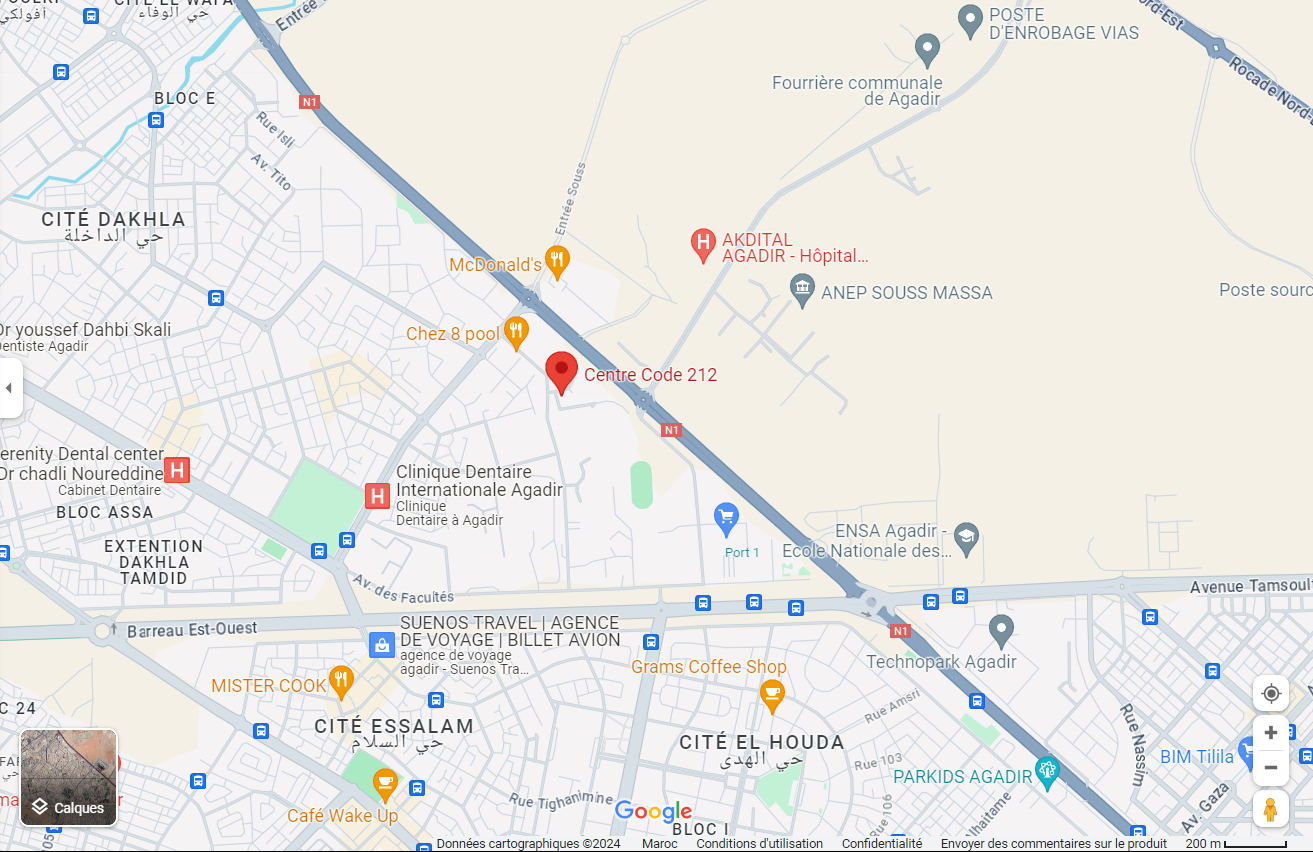
\includegraphics[height=10cm , width=\textwidth]{maps.png}
\caption{Localisation du centre}
\label{fig:localisationcentre}
\end{figure}




\subsection{Domaine d'activites :}

\subsubsection{education et Pedagogie :}
L'education et la pedagogie au sein des centres Code 212 se focalisent sur la fourniture d'une formation specialisee en codage et programmation informatique, adoptant une methode d'enseignement innovante basee sur le peer-to-peer. Cette approche encourage les etudiants à apprendre les uns des autres dans un cadre collaboratif, sans dependance à un enseignement centralise traditionnel, favorisant ainsi l'autonomie et le developpement de competences pratiques en resolution de problèmes. Avec l'ouverture de ces centres, telle celle à l'Universite Ibn Zohr d'Agadir, les etudiants auront accès à une education de pointe en technologie, preparant la nouvelle generation à relever les defis de l'ère numerique et à contribuer activement au marche du travail dans le domaine de l'informatique.

\subsubsection{Renforcement des competences et employabilite :}
Code 212 est dedie à renforcer les competences digitales des etudiants marocains, favorisant ainsi leur employabilite dans un marche en pleine digitalisation. Grâce à des plateformes d'apprentissage interactives et des simulateurs d'examens, les etudiants pratiquent et valident leurs connaissances dans des conditions realistes, les preparant à repondre aux exigences des emplois actuels. Le centre s'engage à tracer un chemin clair pour ses etudiants vers des carrières numeriques florissantes, en leur donnant les outils pour innover et exceller dans une economie de plus en plus axee sur les technologies numeriques.


\thechapter{Presentation du projet :}

\section{Problematique et presentation du projet}
Avec la montee en puissance de la digitalisation, les etablissements educatifs doivent constamment s'adapter pour offrir à leurs etudiants des outils adaptes à leur reussite. Face à cet imperatif, Code 212 a identifie le besoin d'assurer une interaction constante et personnalisee afin de repondre efficacement aux questions frequentes des etudiants et de les assister dans leur parcours educatif.

\subsection{Contexte d'Apprentissage Numerique}
Le contexte actuel de l'education est marque par un passage rapide au numerique. Cela requiert des moyens d'apprentissage qui soient non seulement flexibles mais aussi immediatement reactifs aux besoins des elèves.

\subsection{Besoin d'une Interaction Continue}
À l'ère du numerique, où l'immediatete est devenue la norme, les etudiants s'attendent à obtenir rapidement des reponses à leurs questions. Un outil tel qu'un chatbot IA s'avère indispensable pour combler cet ecart entre les besoins des etudiants et les ressources disponibles.

\section{Solution Proposee}
Le chatbot IA represente une innovation centrale pour Code 212. Capable de dialoguer avec les etudiants en temps reel, il offre une assistance instantanee tout en optimisant les ressources pedagogiques du centre.

\subsection{Le Chatbot IA}
Le chatbot, dote d'intelligence artificielle, est programme pour comprendre et traiter les demandes des etudiants, fournissant des reponses claires et precises, et est même capable d'apprendre de ses interactions pour ameliorer continuellement son assistance.

\subsection{Methodes de Developpement du Chatbot}
Lors du developpement du chatbot, nous avions deux options principales : le fine-tuning et le Retrieval-Augmented Generation (RAG). Après une analyse approfondie des avantages et des inconvenients de chaque methode, nous avons opte pour la methode RAG.

\subsubsection{Le Fine-Tuning}
Le fine-tuning consiste à adapter un modèle de langage pre-entraîne à des tâches specifiques en le re-entraînant sur un ensemble de donnees supplementaires pertinentes.

\paragraph{Avantages du Fine-Tuning}
\begin{itemize}
    \item \textbf{Adaptation specifique}: Permet d’adapter le modèle aux besoins precis en utilisant des donnees specifiques à notre domaine.
    \item \textbf{Amelioration des performances}: Peut ameliorer la precision du modèle pour des tâches specifiques en integrant des nuances et des contextes particuliers.
\end{itemize}

\paragraph{Inconvenients du Fine-Tuning}
\begin{itemize}
    \item \textbf{Coût en ressources}: Le processus de fine-tuning peut être coûteux en termes de calcul et de temps, necessitant des ressources materielles importantes.
    \item \textbf{Dependance aux donnees}: La qualite des resultats depend fortement de la qualite et de la quantite des donnees disponibles pour le re-entraînement.
    \item \textbf{Maintenance complexe}: Necessite une mise à jour continue et une maintenance pour integrer les nouvelles informations et rester pertinent.
\end{itemize}

\subsubsection{Le Retrieval-Augmented Generation (RAG)}
RAG combine un modèle de recuperation d'informations et un modèle de generation de texte. Il fonctionne en recuperant des passages pertinents d'une base de donnees et en generant des reponses en s'appuyant sur ces passages.

\paragraph{Avantages du RAG}
\begin{itemize}
    \item \textbf{Accès à une large base de connaissances}: RAG permet d'acceder à une base de donnees etendue pour recuperer les informations les plus pertinentes, offrant ainsi des reponses plus precises et à jour.
    \item \textbf{Reduction des coûts de calcul}: etant donne que le modèle genère des reponses basees sur des informations recuperees, il necessite moins de re-entraînement intensif, ce qui reduit les coûts en calcul et en temps.
    \item \textbf{Scalabilite et flexibilite}: Facile à mettre à jour avec de nouvelles informations sans necessiter un re-entraînement complet du modèle.
\end{itemize}

\paragraph{Inconvenients du RAG}
\begin{itemize}
    \item \textbf{Complexite de mise en œuvre}: Integrer et optimiser un système RAG peut être plus complexe initialement par rapport au fine-tuning simple d'un modèle.
    \item \textbf{Dependance à la base de donnees}: La qualite des reponses depend de la qualite et de la couverture de la base de donnees utilisee pour la recuperation des informations.
\end{itemize}

\subsubsection{Pourquoi Nous Avons Choisi le RAG}
Nous avons choisi la methode RAG en raison de ses nombreux avantages strategiques. La capacite d'acceder à une vaste base de connaissances et de fournir des reponses precises et actualisees etait cruciale pour nous. De plus, la reduction des coûts de calcul et la flexibilite de mise à jour ont ete des facteurs determinants, permettant une maintenance plus aisee et des mises à jour regulières sans necessiter un re-entraînement complet. Bien que la mise en œuvre initiale ait ete plus complexe, les benefices à long terme en termes de scalabilite et d'efficacite ont justifie notre choix pour la methode RAG.


\section{Tableau des fonctionnalitees}
Nous presentons ici un tableau decrivant les solutions offertes par le chatbot et leur impact sur l'experience des etudiants.


\begin{table}[h!]
\centering
\begin{tabular}{|p{6cm}|p{10cm}|}
\hline
\textbf{Fonctionnalite} & \textbf{Description et Impact sur les etudiants} \\ \hline
Reponses aux questions frequentes & Le chatbot fournit des reponses immediates aux interrogations des etudiants, facilitant l'apprentissage autonome et une meilleure comprehension des cours. \\ \hline
Assistance pour les travaux pratiques & Il guide les etudiants dans la realisation de leurs travaux pratiques en offrant des conseils et des ressources utiles, ce qui contribue à approfondir leur comprehension et à ameliorer leur competence pratique. \\ \hline
Gestion des ressources pedagogiques & Le chatbot aide à la navigation et à l'exploitation efficace des ressources pedagogiques mises à disposition, maximisant ainsi le temps d'etude et les resultats d'apprentissage. \\ \hline
Support psychologique & À travers des interactions engageantes et empathiques, le chatbot peut proposer un soutien moral et motiver les etudiants, renforçant leur perseverance et leur engagement scolaire. \\ \hline
\end{tabular}
\caption{Recapitulatif des fonctionnalites du chatbot IA et leur impact sur les etudiants de Code 212.}
\label{tab:chatbotfeatures}
\end{table}

\section{Conduite du Projet}
La conduite efficace du projet de developpement du chatbot IA est essentielle pour repondre aux exigences specifiques de Code 212. Cette section explore en detail les processus de conception, de planification et de developpement qui sous-tendent la creation du chatbot.

\subsection{Conception}
La phase de conception est l'etape fondatrice du projet, où l'equipe fixe les objectifs du chatbot, identifie les fonctionnalites cles et elabore la structure generale de l'intelligence artificielle. Cette phase necessite une comprehension precise des besoins des etudiants qui seront les utilisateurs finaux. À ce stade, des ateliers de brainstorming, des enquêtes auprès des utilisateurs et des seances de feedback avec les principales parties prenantes sont utilises pour rassembler les exigences et pour esquisser les premiers prototypes de l'interface utilisateur. Les scenarios d'utilisation et les parcours utilisateurs sont meticuleusement elabores pour garantir que le chatbot est à la fois convivial et techniquement viable.

\subsection{Planification des Tâches}
Une planification detaillee va de pair avec une conception reussie; elle s'attaque à la complexite du processus de developpement en ventilant le projet en petites tâches gerables. L'equipe du projet etablit un calendrier de realisation, determinant les dependances entre les tâches et en allouant les ressources necessaires. La methodologie Agile est souvent adoptee, permettant une flexibilite et une reactivite accrues face aux changements de scope ou aux retours des utilisateurs. La creation de sprints, la priorisation des backlogs et les revues regulières de sprint assurent que le projet reste sur la bonne voie et adapte aux exigences changeantes tout au long de son cycle de vie.

\subsection{Developpement et Integrations}
Durant la phase de developpement, l'equipe met en œuvre la conception du chatbot en codant les differentes composantes logicielles. Les developpeurs intègrent l'intelligence artificielle, travaillent sur le traitement du langage naturel et l'apprentissage automatique pour offrir une experience utilisateur la plus authentique possible. La construction de l'infrastructure technique, comprenant des serveurs, des bases de donnees et l'integration avec les API existantes, est rigoureusement testee pour garantir son bon fonctionnement. Une serie exhaustive de tests—tests unitaires, tests d'integration et tests de charge—est realisee pour s'assurer que le système est robuste, evolutif et prêt pour le deploiement.
Chacune de ces etapes est critique pour le succès du chatbot IA qui est cense non seulement interagir efficacement avec les utilisateurs mais aussi evoluer avec le centre educatif Code 212 afin d'ameliorer continuellement le support offert aux etudiants.


\section{Methodologie Scrum et ses rôles}

Scrum est une methodologie agile utilisee principalement dans le developpement de logiciels pour gerer des projets complexes et assurer une livraison continue de produits de haute qualite. Elle repose sur des cycles de developpement iteratifs et incrementaux appeles "sprints", qui durent generalement de deux à quatre semaines. Scrum encourage la collaboration, la flexibilite et l'amelioration continue à travers des revues regulières et des retrospectives.

\subsection{Les rôles dans Scrum}

\begin{itemize}
    \item \textbf{Product Owner (PO)} \\
    Le Product Owner est responsable de maximiser la valeur du produit resultant du travail de l'equipe de developpement. Il gère le backlog produit, un document evolutif contenant les exigences et les fonctionnalites du produit, en le priorisant selon la valeur ajoutee pour le client et les parties prenantes.
    
    \item \textbf{Scrum Master} \\
    Le Scrum Master est le facilitateur de l'equipe Scrum. Il s'assure que Scrum est compris et applique correctement, en aidant l'equipe à suivre les pratiques et les principes Scrum. Le Scrum Master elimine les obstacles qui peuvent empêcher l'equipe de progresser et veille à ce que l'equipe fonctionne efficacement.
    
    \item \textbf{equipe de Developpement} \\
    L'equipe de developpement est composee de professionnels qui travaillent ensemble pour livrer des increments de produit potentiellement livrables à la fin de chaque sprint. L'equipe est auto-organisee et interdisciplinaire, possedant toutes les competences necessaires pour accomplir le travail sans dependre d'autres personnes exterieures à l'equipe.
\end{itemize}

\begin{figure}[H]
\centering
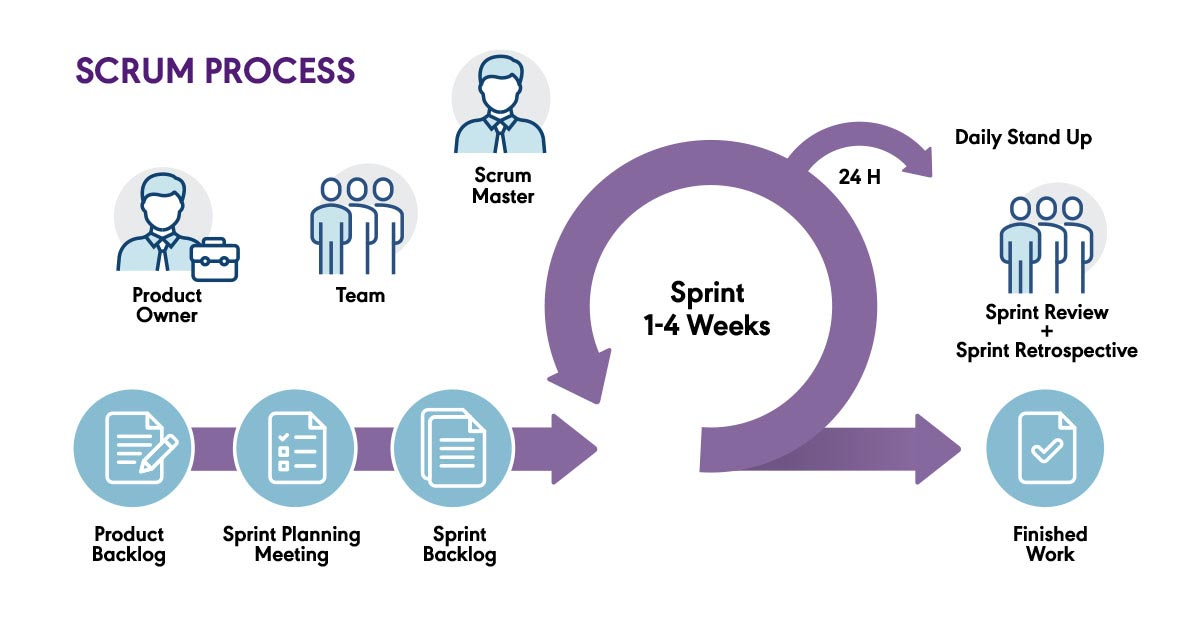
\includegraphics[width=\textwidth]{scrum.jpg}
\caption{Methodologie Scrum}
\label{fig:methodologie_scrum}
\end{figure}



\section{Conclusion}
En conclusion, ce chapitre a mis en lumière la methodologie appliquee dans la conduite du projet de developpement du chatbot IA pour Code 212. L'approche methodique de la conception, la rigueur de la planification des tâches et l'agilite du developpement ont façonne un outil prometteur pour l'enrichissement de l'experience educative des etudiants. La maturite du processus adopte reflète notre engagement envers les valeurs d'excellence, de reactivite aux besoins des utilisateurs et d'innovation constante.

L'interaction entre la technologie de pointe et la pedagogie moderne de Code 212, incarnee par le chatbot IA, est destinee à etablir un nouveau standard en matière d'assistance etudiante en temps reel. Avec la fin de ce chapitre, nous anticipons la transition vers les phases subsequentes de mise en œuvre, d'evaluation et d'optimisation, qui seront abordees dans les chapitres suivants. L'impact positif attendu du chatbot sur l'accès à l'information et l'autonomie des etudiants suggère une transformation significative de leur parcours d'apprentissage numerique.

\chapter{Sprint de preparation}

\section{Introduction}
Ce chapitre presente l'analyse fonctionnelle de l'application web integree et du chatbot IA destines aux etudiants et administrateurs de Code 212. L'objectif est de fournir une plateforme complète et interactive pour la gestion des cours, l'emission de certificats et l'assistance en temps reel via un chatbot intelligent. Cette analyse detaillee etablira des directives pour le developpement d'une interface utilisateur intuitive, mettant en avant les besoins et preferences des utilisateurs, tout en integrant des outils automatises pour une experience pedagogique optimisee. Un système convivial et performant servira de catalyseur pour une meilleure engagement et une acquisition des connaissances plus efficace chez les etudiants.







\section{Identification des Besoins Utilisateurs}
Pour developper une application web et un chatbot IA repondant aux besoins des utilisateurs de Code 212, nous avons entrepris un processus approfondi d'etude de marche, incluant des analyses comportementales, des sondages et des sessions de feedback avec les parties prenantes. Le besoin d'un accès simplifie aux ressources pedagogiques, d'une plateforme flexible pour suivre les cours et obtenir des certificats ainsi que d'une assistance instantanee pour des requêtes diverses sont clairement apparus. L'application web doit faciliter une navigation fluide et une gestion transparente du contenu des cours, tandis que le chatbot IA doit completer cette experience en guidant les utilisateurs à travers les fonctionnalites et en repondant aux questions academiques et administratives.

% Inserez ici un tableau qui resume les besoins des utilisateurs pour l'application web et le chatbot.
\begin{table}[htp]
\caption{Besoins utilisateurs pour l'application web et le chatbot IA}
\centering
\begin{tabular}{|m{4cm}|m{12cm}|}
\hline
\textbf{Besoin identifie} & \textbf{Description du besoin} \\ \hline
Gestion intuitive des cours & L'application doit offrir une interface permettant aux etudiants de s'inscrire facilement aux cours, de suivre leur progression et d'acceder au materiel de cours. \\ \hline
Delivrance des certificats & Un système automatise pour la demande et l'obtention de certificats après la reussite des evaluations est necessaire pour valider les competences acquises. \\ \hline
Assistance en continu & Le chatbot IA doit être disponible 24/7 pour repondre aux questions concernant l'utilisation de l'application, la navigation entre les cours, ainsi que les processus de certification. \\ \hline
% Ajoutez d'autres besoins identifies ici.
\end{tabular}
\label{tab:user_needs}
\end{table}

En repondant à ces besoins, l'application web et le chatbot IA representent un environnement d'apprentissage complet et integre, qui favorise l'excellence educative et l'independance des etudiants de Code 212.

%Cette introduction et la table des besoins des utilisateurs fournissent une vue d'ensemble qui pave la voie pour developper le reste de l'analyse fonctionnelle, la conception de l'application et l'implementation du chatbot.


\section{Specification des Fonctionnalites}
La specification des fonctionnalites traduit les besoins utilisateurs en caracteristiques techniques et operationnelles concrètes de l'application et du chatbot. Cette section detaille les fonctionnalites essentielles requises pour repondre aux exigences des etudiants et des administrateurs de Code 212.

% Un tableau pourrait être utilise pour lister et decrire les fonctionnalites
\begin{table}[htp]
\caption{Specification des fonctionnalites de l'application web et du chatbot IA}
\centering
\begin{tabular}{|m{4cm}|m{5cm}|m{7cm}|}
\hline
\textbf{Fonctionnalite} & \textbf{Composant} & \textbf{Description} \\ \hline
Inscription aux Cours & Application web & Permet aux utilisateurs de s'inscrire et de se desinscrire facilement des cours offerts par Code 212. \\ \hline
Suivi de Progression & Application web & Affiche la progression de l'apprenant dans chaque cours et enregistre les jalons academiques atteints. \\ \hline
Assistance & Chatbot IA & Repond aux questions des utilisateurs concernant la navigation de l'application et les problèmes techniques ou administratifs. \\ \hline
% Ajoutez d'autres fonctionnalites specifiques au projet.
\end{tabular}
\label{tab:functional_specs}
\end{table}

Ces fonctionnalites doivent être developpees en tenant compte des meilleures pratiques de l'UX/UI pour assurer une facilite d'utilisation et engager activement les utilisateurs avec l'application.

\section{Besoins non fonctionnels}

Pour completer les besoins fonctionnels, notre projet devra respecter quelques proprietes contribuant à une meilleure qualite de la solution obtenue. Parmi ces critères, on retrouve :

\begin{itemize}
    \item \textbf{Performance} : Il s'agit d'optimiser le temps de chargement des donnees ainsi que d'utiliser les bonnes pratiques du developpement.
    \item \textbf{evolutivite} : L'application doit pouvoir integrer de nouvelles extensions en ajoutant des modules pour repondre aux nouveaux besoins fonctionnels, sans modifier les modules dejà existants.
    \item \textbf{Securite} : L'accès à l'application et aux donnees doit être securise. Pour gerer les autorisations aux differents modules de l'application, nous avons utilise Spring Security.
    \item \textbf{Haute disponibilite} : L'application doit être disponible en permanence, minimisant les temps d'arrêt et assurant un fonctionnement continu même en cas de defaillance d'une partie du système.
\end{itemize}


\section{Fonctionalitees attendues}

Les cas d'utilisation detailles illustrent les interactions typiques entre les utilisateurs et l'application, couvrant aussi bien les fonctionnalites du site web que celles du chatbot. Ils permettent de visualiser les scenarios quotidiens et d'identifier les points de contact entre l'utilisateur et le système.

\subsection{Inscription à un cours via l'application web}
\textbf{Acteurs:} etudiant \\
\textbf{Prerequis:} L'etudiant est connecte à son compte. \\
\textbf{Scenario principal:}
\begin{enumerate}
    \item L'etudiant selectionne l'option 'Catalogue de Cours' dans le menu.
    \item Il recherche et selectionne le cours souhaite.
    \item Il lit les details du cours et verifie les prerequis.
    \item L'etudiant s'inscrit au cours en cliquant sur 'S'inscrire'.
    \item Le système enregistre l'inscription et met à jour l'espace personnel de l'etudiant.
\end{enumerate}

\subsection{Inscription à un evenement via l'application web}
\textbf{Acteurs:} etudiant \\
\textbf{Prerequis:} L'etudiant est connecte à son compte. \\
\textbf{Scenario principal:}
\begin{enumerate}
    \item L'etudiant selectionne l'option 'evenements' dans le menu.
    \item Il recherche et selectionne l'evenement souhaite.
    \item Il lit les details de l'evenement et verifie les informations pertinentes.
    \item L'etudiant s'inscrit à l'evenement en cliquant sur 'S'inscrire'.
    \item Le système enregistre l'inscription et met à jour l'espace personnel de l'etudiant.
\end{enumerate}

\subsection{Demande de certificat via le chatbot IA}
\textbf{Acteurs:} etudiant, Chatbot IA \\
\textbf{Prerequis:} L'etudiant a termine le cours avec succès. \\
\textbf{Scenario principal:}
\begin{enumerate}
    \item L'etudiant demande au chatbot la procedure pour obtenir un certificat.
    \item Le chatbot fournit les etapes à suivre et demande si l'etudiant souhaite proceder.
    \item Après confirmation, le chatbot initie la procedure de demande de certificat dans le système.
    \item L'etudiant est guide à travers le processus et soumet sa demande.
    \item Le chatbot confirme que la demande a ete soumise et indique le delai de traitement.
\end{enumerate}

\subsection{Gestion des evenements, cours et certificats par le gestionnaire}
\textbf{Acteurs:} Gestionnaire \\
\textbf{Prerequis:} Le gestionnaire est connecte à son compte administrateur. \\
\textbf{Scenario principal:}
\begin{enumerate}
    \item Le gestionnaire selectionne l'option 'Gestion des evenements' dans le menu.
    \item Il ajoute, supprime ou modifie les informations des evenements selon les besoins.
    \item Le gestionnaire accède à la section 'Gestion des Cours' pour ajouter, supprimer ou modifier les cours disponibles.
    \item Il navigue vers 'Gestion des Certificats' pour administrer les demandes de certificats, en ajoutant ou en supprimant des certificats selon les demandes des etudiants.
    \item Le système enregistre les modifications et met à jour les informations correspondantes dans la base de donnees.
\end{enumerate}

\subsection{Gestion des utilisateurs par l'administrateur}
\textbf{Acteurs:} Administrateur \\
\textbf{Prerequis:} L'administrateur est connecte à son compte administrateur. \\
\textbf{Scenario principal:}
\begin{enumerate}
    \item L'administrateur selectionne l'option 'Gestion des Utilisateurs' dans le menu.
    \item Il consulte la liste des utilisateurs inscrits sur la plateforme.
    \item L'administrateur ajoute, supprime ou modifie les informations des utilisateurs selon les besoins.
    \item Le système enregistre les modifications et met à jour les informations correspondantes dans la base de donnees.
\end{enumerate}

Ces cas d'utilisation representent des interactions frequentes et essentielles qui doivent être prises en compte pour une experience utilisateur coherente et satisfaisante. Ils permettent egalement de detecter les points potentiels d'amelioration dans le processus d'interaction.



\section{Backlog Produit}

Le developpement de notre application microservices s'est structure autour d'un backlog produit bien defini, comprenant plusieurs epopees et user stories. Chaque user story a ete accompagnee de critères d'acceptation clairs pour garantir la qualite et la conformite aux attentes.

\subsection{epopee 1 : Developpement et Integration du Chatbot}

\textbf{User Story 1.1 : Configuration Initiale du Chatbot}
\begin{itemize}
    \item \textbf{En tant que} developpeur
    \item \textbf{Je veux} configurer le cadre initial du chatbot
    \item \textbf{Afin de} disposer d'une base solide sur laquelle construire
    \item \textbf{Critères d'acceptation :}
    \begin{itemize}
        \item Le cadre du chatbot est configure et integre dans la plateforme.
        \item Les capacites conversationnelles de base sont mises en place.
    \end{itemize}
\end{itemize}

\textbf{User Story 1.2 : Base de Connaissances du Chatbot}
\begin{itemize}
    \item \textbf{En tant que} utilisateur
    \item \textbf{Je veux} poser des questions au chatbot sur Code212
    \item \textbf{Afin de} recevoir des informations specifiques sur l'ecole
    \item \textbf{Critères d'acceptation :}
    \begin{itemize}
        \item Le chatbot peut repondre avec precision aux questions sur Code212.
        \item La base de connaissances comprend des informations sur les cours, les evenements et les examens de certification.
    \end{itemize}
\end{itemize}

\textbf{User Story 1.3 : Mise à Jour de la Base de Donnees par l'Administrateur}
\begin{itemize}
    \item \textbf{En tant que} administrateur
    \item \textbf{Je veux} pouvoir mettre à jour la base de donnees du chatbot à tout moment
    \item \textbf{Afin de} m'assurer que les informations sont toujours à jour
    \item \textbf{Critères d'acceptation :}
    \begin{itemize}
        \item L'administrateur peut acceder à une interface pour mettre à jour la base de donnees.
        \item Les modifications sont immediatement refletees dans les reponses du chatbot.
    \end{itemize}
\end{itemize}

\subsection{epopee 2 : Developpement des Fonctionnalites de la Plateforme}

\textbf{User Story 2.1 : Consultation des Cours Disponibles}
\begin{itemize}
    \item \textbf{En tant que} utilisateur
    \item \textbf{Je veux} voir la liste des cours disponibles
    \item \textbf{Afin de} choisir ceux qui m'interessent
    \item \textbf{Critères d'acceptation :}
    \begin{itemize}
        \item Une liste des cours disponibles est affichee.
        \item Les details de chaque cours sont accessibles.
    \end{itemize}
\end{itemize}

\textbf{User Story 2.2 : Inscription aux Cours et evenements}
\begin{itemize}
    \item \textbf{En tant que} utilisateur
    \item \textbf{Je veux} m'inscrire aux cours et evenements
    \item \textbf{Afin de} participer à ceux-ci
    \item \textbf{Critères d'acceptation :}
    \begin{itemize}
        \item Les utilisateurs peuvent s'inscrire à des cours et des evenements via la plateforme.
        \item Un système de confirmation d'inscription est en place.
    \end{itemize}
\end{itemize}

\textbf{User Story 2.3 : Inscription aux Examens de Certification Gratuits}
\begin{itemize}
    \item \textbf{En tant que} utilisateur
    \item \textbf{Je veux} m'inscrire à des examens de certification gratuits
    \item \textbf{Afin de} obtenir des certifications
    \item \textbf{Critères d'acceptation :}
    \begin{itemize}
        \item Les utilisateurs peuvent voir les examens de certification disponibles et s'y inscrire gratuitement.
        \item Un système de confirmation d'inscription aux examens est en place.
    \end{itemize}
\end{itemize}

\subsection{epopee 3 : Ameliorations et Optimisations}

\textbf{User Story 3.1 : Amelioration de l'Interface Utilisateur}
\begin{itemize}
    \item \textbf{En tant que} utilisateur
    \item \textbf{Je veux} une interface utilisateur intuitive et conviviale
    \item \textbf{Afin de} naviguer facilement sur la plateforme
    \item \textbf{Critères d'acceptation :}
    \begin{itemize}
        \item L'interface utilisateur est testee et optimisee pour une meilleure experience utilisateur.
        \item Les utilisateurs fournissent des retours positifs sur la convivialite.
    \end{itemize}
\end{itemize}

\textbf{User Story 3.2 : Optimisation des Performances du Chatbot}
\begin{itemize}
    \item \textbf{En tant que} developpeur
    \item \textbf{Je veux} optimiser les performances du chatbot
    \item \textbf{Afin de} garantir des reponses rapides et precises
    \item \textbf{Critères d'acceptation :}
    \begin{itemize}
        \item Le temps de reponse du chatbot est reduit.
        \item La precision des reponses du chatbot est amelioree.
    \end{itemize}
\end{itemize}

\subsection{Sprint Plan}

\textbf{Sprint 1:} Planification et configuration initiale du chatbot (User Story 1.1), Base de connaissances du chatbot (User Story 1.2)

\textbf{Sprint 2:} Authentification et mise à jour de la base de donnees par l'administrateur (User Story 1.3), Consultation des cours disponibles (User Story 2.1)

\textbf{Sprint 3:} Inscription aux cours et evenements (User Story 2.2), Inscription aux examens de certification gratuits (User Story 2.3)

\textbf{Sprint 4:} Amelioration de l'interface utilisateur (User Story 3.1), Optimisation des performances du chatbot, deploiment et creation des contenaires (User Story 3.2)


\section{PLANIFICATION DU PROJET}
Le diagramme de Gantt suivant presente le planning du projet, indiquant les differentes phases de developpement et les delais associes.



\subsection{PLANNING PREVISIONNEL}

\begin{figure}[h!]
\centering
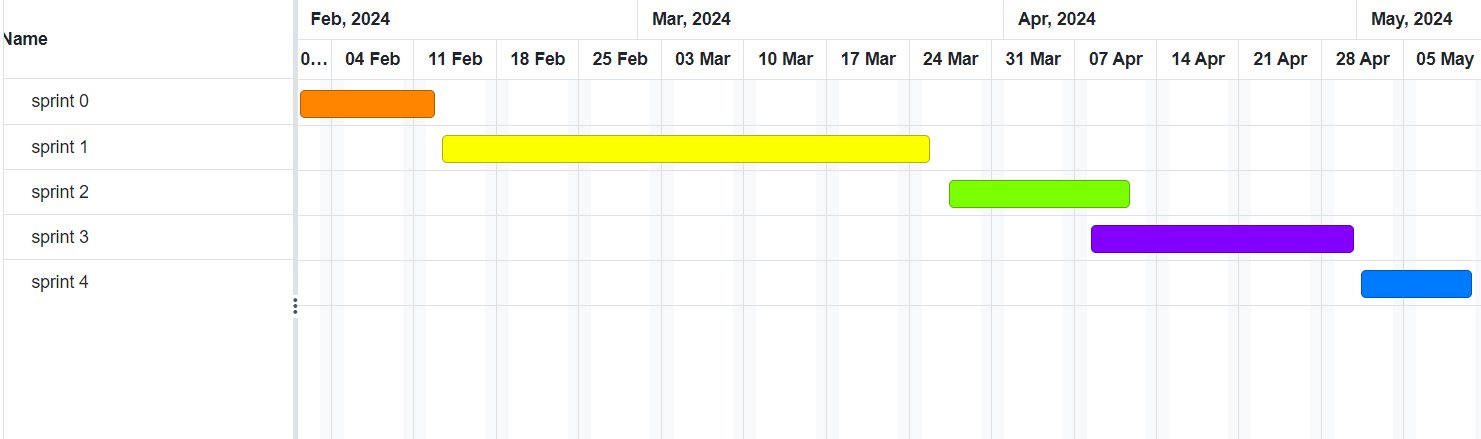
\includegraphics[width=\textwidth]{gant-prev.png}
\caption{Diagramme de Gantt previsionnel.}
\label{fig:prev-gantt}
\end{figure}


\clearpage





\subsection{PLANNING REEL}

\begin{figure}[h!]
\centering
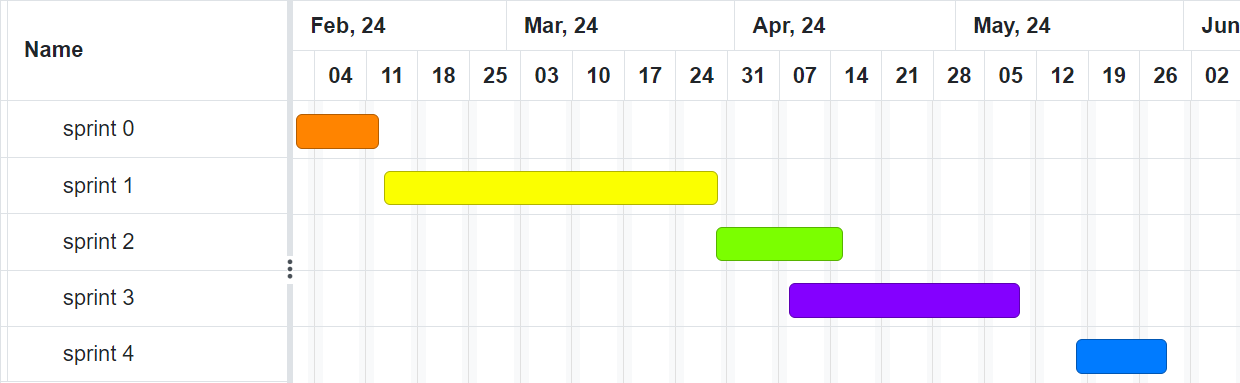
\includegraphics[width=\textwidth]{gantt-reel.png}
\caption{Diagramme de Gantt reele.}
\label{fig:reel-gantt}
\end{figure}
\clearpage
\section{Diagramme de Cas d'Utilisation globale}
Le diagramme de cas d'utilisation offre une representation graphique des fonctionnalites du système telles qu'elles sont experimentees par les differents acteurs. Il identifie les interactions entre l'utilisateur (etudiant, administrateur) et le système et illustre les principaux scenarios d'utilisation. 
\clearpage

\begin{figure}[h!]

\centering
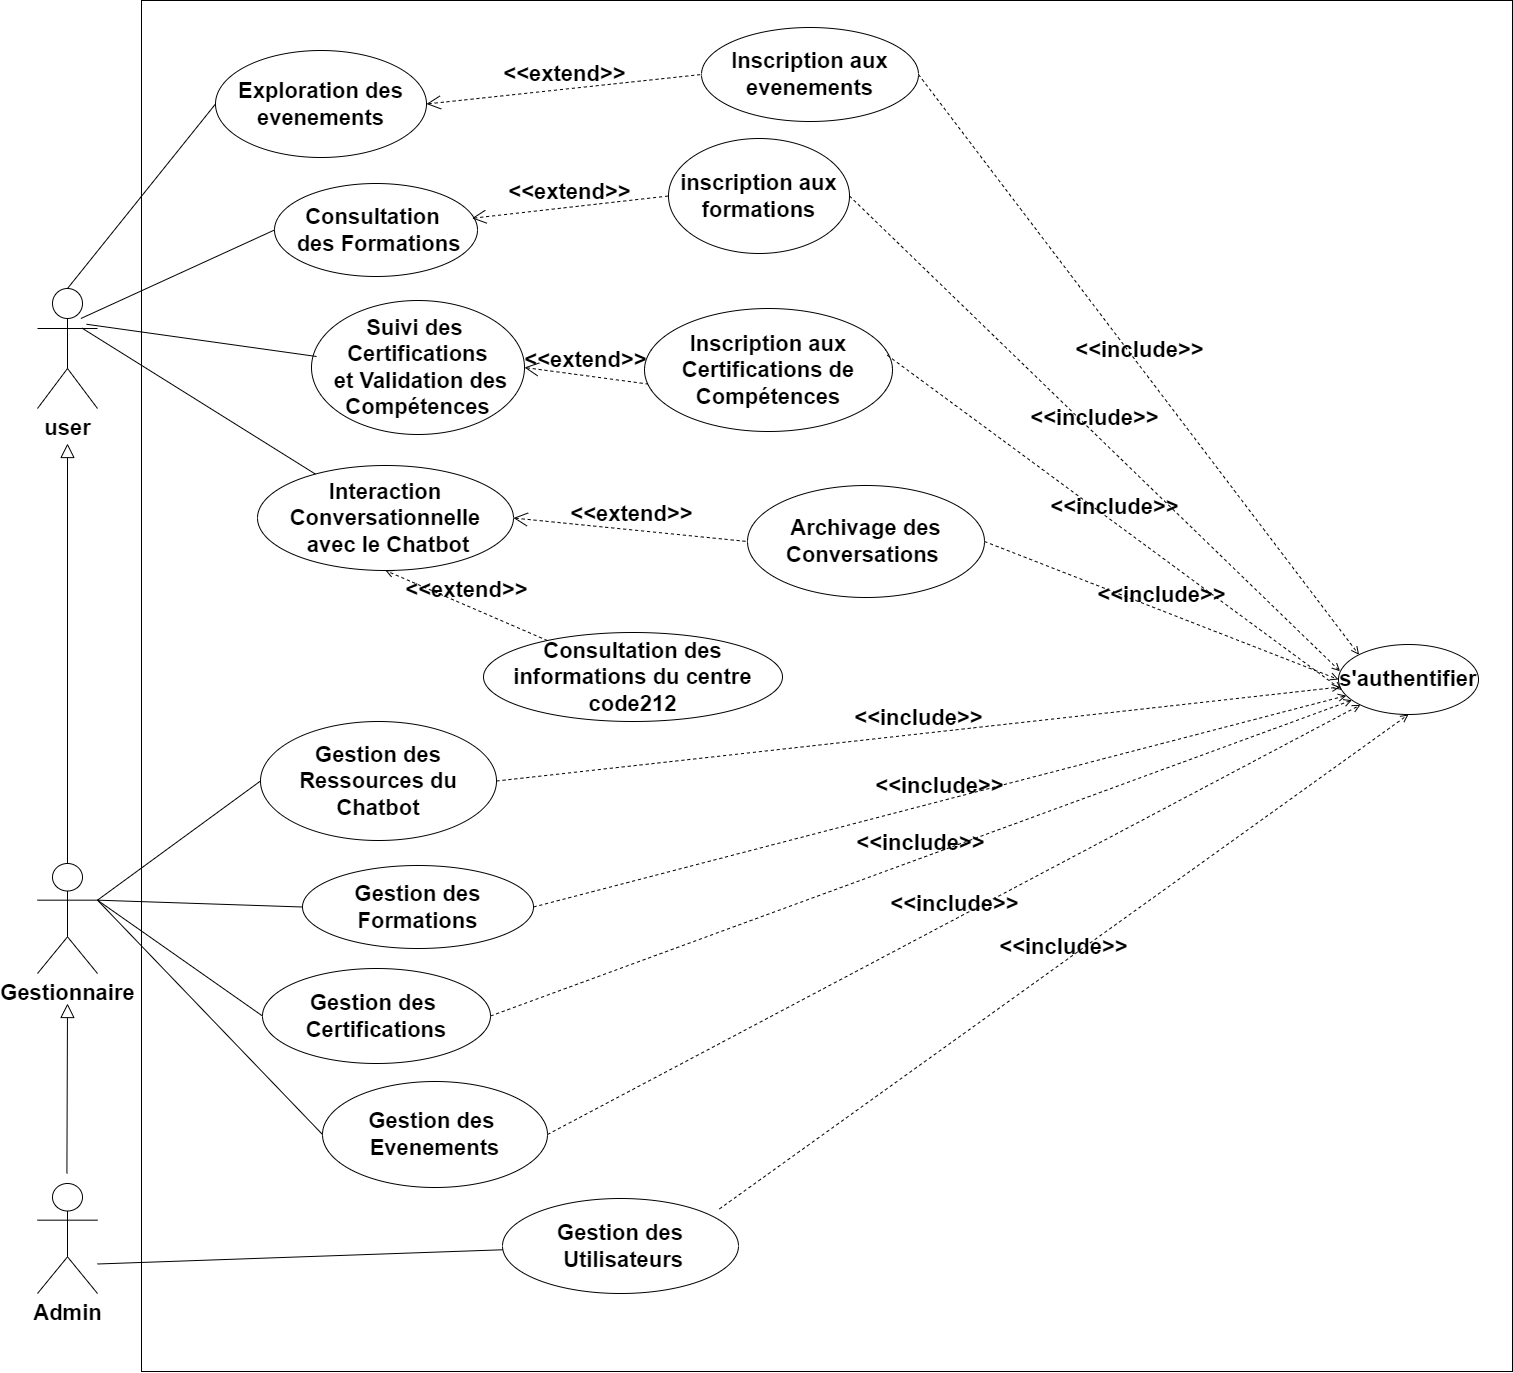
\includegraphics[width=\textwidth]{images/usecase.png}
\caption{Diagramme de cas d'utilisation pour l'application web et le chatbot IA.}
\label{fig:use_case_diagram}
\end{figure}



\section{Diagramme de Classes globale}

Le diagramme de classes est essentiel pour visualiser la structure statique de l'application et decrire les objets encapsules dans le système ainsi que leurs relations. Il fournit une vue d'ensemble des classes, de leurs attributs, methodes et des associations inter-classes qui modelisent les donnees de l'application.

% Incluez votre diagramme de classes ici
% Incluez votre diagramme de classes ici
\clearpage
\begin{figure}[h!]
\centering
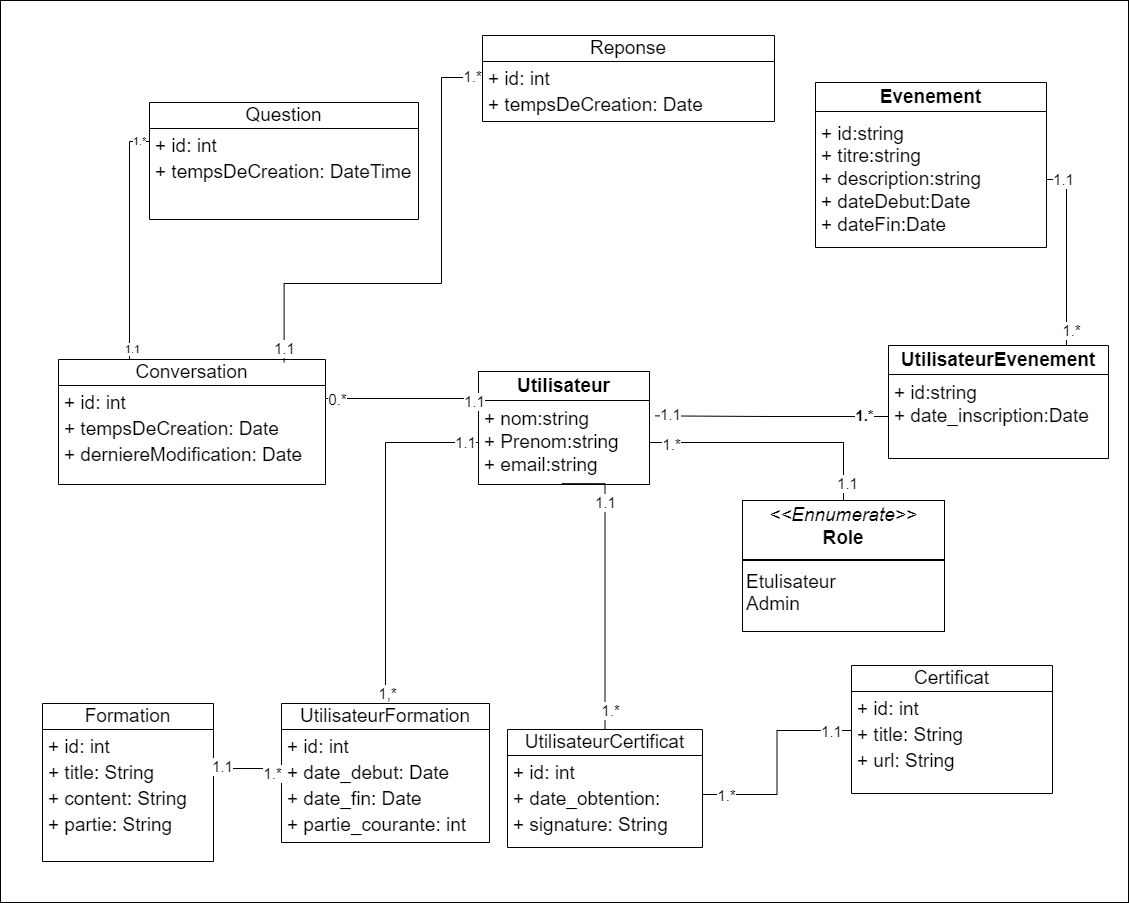
\includegraphics[width=\textwidth]{images/class.png}
\caption{Diagramme de classes pour l'application web et le chatbot IA.}
\label{fig:class_diagram}
\end{figure}

\section{Conclusion de Conception}
La conception de l'application web et du chatbot IA suppose la creation d'une architecture robuste et evolutif qui repond aux besoins fonctionnels tout en offrant une experience utilisateur transparente et engageante. Les diagrammes et modèles presentes dans ce chapitre constituent le socle pour les developpements futurs et pour l'implementation du système.

% Pensez à actualiser les chemins d'accès aux images des diagrammes avec les chemins reels de vos fichiers.
% De plus, adaptez le contenu textuel pour refleter les specificites de votre application et du chatbot.




\chapter{etude Technique}

\section{Introduction}
Ce chapitre presente une etude technique detaillee de l'application basee sur une architecture de microservices. L'architecture est conçue pour assurer une modularite, une evolutivite et une gestion efficace des services. L'application comprend trois principaux microservices : un service REST pour le chatbot IA, un service Spring pour le gateway et proxy, et un service Keycloak pour la gestion des identites et des accès. Cette etude couvre l'architecture des microservices, les technologies utilisees, les interactions entre les services et les choix de conception pour garantir une performance et une securite optimales.

\section{Architecture des Microservices}

L'architecture de l'application est basee sur des microservices, où chaque service est conçu pour être independant et interagir avec les autres services via des API bien definies. Cette section decrit l'architecture globale, les rôles specifiques de chaque service, ainsi que les benefices qu'offre une architecture basee sur les microservices.

\subsection{Description de l'Architecture}

L'architecture de notre projet est divisee en plusieurs services independants. Chaque service est responsable d'une fonctionnalite specifique et communique avec les autres services par le biais de protocoles de communication legers comme HTTP/REST ou gRPC. Cette approche permet une meilleure modularite et une maintenance facilitee de l'application.




\newpage



\subsection{L'Architecture du projet}

\begin{figure}[H] % Utiliser [H] pour forcer l'emplacement
\centering
\rotatebox{90}{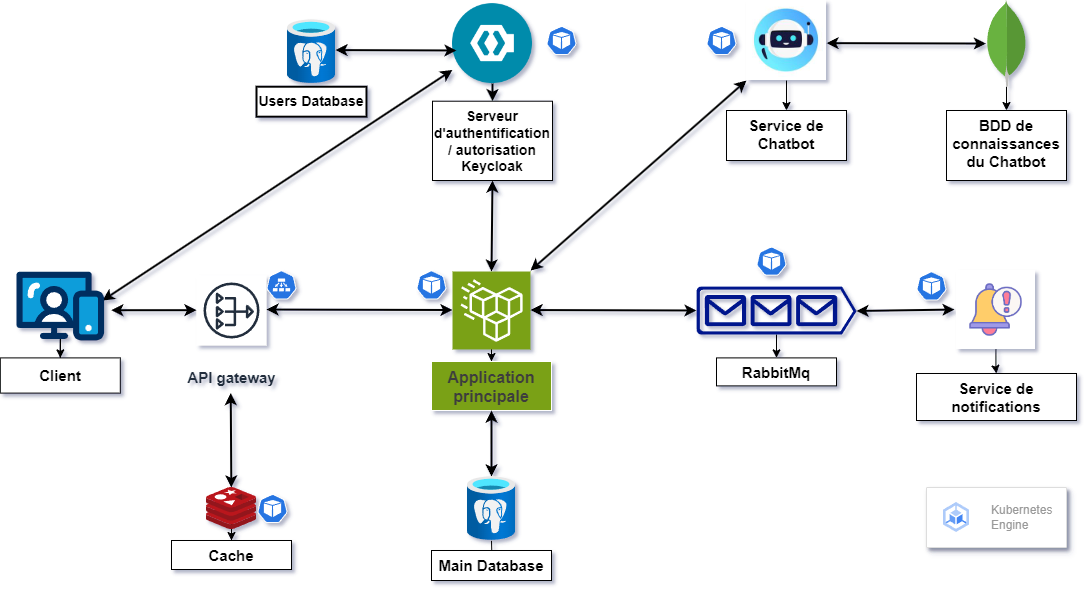
\includegraphics[width=1.5\textwidth]{images/architecture.png}} % Remplacez par le chemin de votre diagramme d'architecture
\caption{Diagramme de l'architecture des microservices}
\label{fig:microservices_architecture}
\end{figure}


\subsection{Description des Services}
\begin{itemize}
    \item \textbf{Service 1 : REST Chatbot IA}
    \begin{itemize}
        \item \textbf{Technologie :} Node.js, Express
        \item \textbf{Fonctionnalite :} Ce service est responsable de traiter les requêtes liees au chatbot IA. Il utilise des techniques de traitement du langage naturel (NLP) et d'apprentissage automatique pour fournir des reponses intelligentes aux utilisateurs.
        \item \textbf{Endpoints principaux :}
        \begin{itemize}
            \item \texttt{GET /chatbot/message} : Recuperer les messages du chatbot.
            \item \texttt{POST /chatbot/message} : Envoyer un message au chatbot et recevoir une reponse.
        \end{itemize}
    \end{itemize}
    
    \item \textbf{Service 2 : Spring Gateway et Proxy}
    \begin{itemize}
        \item \textbf{Technologie :} Spring Boot, Spring Cloud Gateway
        \item \textbf{Fonctionnalite :} Ce service agit comme une passerelle pour les autres microservices, gerant le routage, la gestion des API, et servant de proxy pour les demandes des utilisateurs. Il centralise les appels aux microservices et offre des fonctionnalites telles que le load balancing, le logging, et la securite.
        \item \textbf{Endpoints principaux :}
        \begin{itemize}
            \item \texttt{GET /api/*} : Route les requêtes vers les services appropries.
            \item \texttt{POST /api/*} : Gère les requêtes POST en les acheminant vers les microservices correspondants.
        \end{itemize}
    \end{itemize}
    
    \item \textbf{Service 3 : Keycloak}
    \begin{itemize}
        \item \textbf{Technologie :} Keycloak
        \item \textbf{Fonctionnalite :} Keycloak est utilise pour la gestion des identites et des accès, offrant des fonctionnalites telles que l'authentification, l'autorisation, la gestion des utilisateurs, et la federation des identites. Il securise les endpoints des autres microservices et gère les sessions utilisateurs.
        \item \textbf{Endpoints principaux :}
        \begin{itemize}
            \item \texttt{/auth} : Point de terminaison principal pour les operations d'authentification et de gestion des utilisateurs.
        \end{itemize}
    \end{itemize}
\end{itemize}







\section{Communication entre les Services}
La communication entre les microservices est principalement assuree via des API RESTful et Kafka. Le service Spring Gateway agit comme un point d'entree unique pour toutes les requêtes des utilisateurs et distribue ces requêtes aux services appropries. Keycloak assure la securite des communications en authentifiant les utilisateurs et en autorisant les requêtes.

\subsection{Communication via API RESTful}
Les API RESTful sont utilisees pour les interactions synchrones entre les microservices. Chaque service expose des endpoints specifiques pour recevoir et traiter les requêtes, assurant ainsi une communication claire et structuree. Le Spring Gateway reçoit les requêtes des utilisateurs, applique les règles de routage et transmet les requêtes aux microservices correspondants.

\subsection{Communication via Kafka}
Kafka est utilise pour la communication asynchrone entre les microservices. Les evenements importants, tels que les mises à jour de donnees ou les notifications, sont publies dans des topics Kafka. Les microservices abonnes à ces topics peuvent consommer les messages et effectuer les actions necessaires. Cette approche permet de decoupler les services et d'assurer une meilleure scalabilite et resilience.

\section{Choix de Conception et Justifications}
\subsection{Microservices vs Monolithique}
L'architecture microservices a ete choisie pour sa modularite et son evolutivite. Contrairement à une architecture monolithique, les microservices permettent un developpement, un deploiement et une maintenance independants des composants de l'application.

\subsection{Securite avec Keycloak}
Keycloak est utilise pour securiser les microservices. Il offre des fonctionnalites avancees telles que l'authentification unique (SSO), la federation des identites, et la gestion fine des autorisations, assurant une securite robuste et centralisee.

\subsection{Scalabilite et Resilience}
L'utilisation de Spring Cloud Gateway permet de gerer efficacement le trafic reseau et de distribuer la charge de manière equilibree entre les services. Cela ameliore la scalabilite et la resilience de l'application, garantissant une disponibilite elevee même en cas de pic de trafic.

\section{Conclusion}
Cette etude technique a detaille l'architecture des microservices de l'application, les technologies choisies, et les interactions entre les differents services. L'approche microservices, combinee à l'utilisation de Keycloak pour la gestion des identites et des accès, assure une application modulaire, securisee, et facilement scalable. Les choix de conception visent à offrir une experience utilisateur optimale tout en garantissant la performance et la securite de l'application.
\chapter{Realisation et Mise en Œuvre}

\section{Introduction}
Ce chapitre decrit les etapes de realisation et de mise en œuvre de l'application, detaillant les differentes phases de developpement, les technologies utilisees, et les processus suivis pour garantir le succès du projet. Un diagramme de Gantt est egalement presente pour illustrer le planning du projet et les delais associes à chaque phase.


\section{Utilisation de Redmine}

Redmine a ete un outil central dans la gestion de notre projet. Voici quelques-unes des fonctionnalites cles que nous avons utilisees :

\subsection{Gestion des Tâches}

Nous avons cree des tickets de tâche pour chaque activite à realiser, en les classant par categorie et en les assignant aux membres de l'equipe. Chaque ticket contenait une description detaillee de la tâche, les critères d'acceptation, et une estimation du temps necessaire.

\subsection{Suivi du Temps}

Redmine nous a permis de suivre le temps passe sur chaque tâche, facilitant ainsi la gestion des ressources et l'evaluation de la productivite. Chaque membre de l'equipe enregistrait ses heures de travail quotidiennement.

\subsection{Gantt Chart}

La fonctionnalite de Gantt chart de Redmine a ete particulièrement utile pour visualiser la planification du projet et suivre l'avancement des differentes phases. Nous avons pu identifier rapidement les retards et ajuster les plannings en consequence.

\subsection{Gestion des Bugs}

Lors des phases de developpement et de tests, nous avons utilise Redmine pour suivre les bugs et les anomalies. Chaque bug etait documente avec des etapes de reproduction, des captures d'ecran, et assigne à un developpeur pour correction.

\subsection{Collaboration et Communication}

Redmine a facilite la communication et la collaboration entre les membres de l'equipe. Les commentaires sur les tickets, les notifications par email et les forums de discussion integres ont permis de maintenir une communication fluide et efficace.


\newpage

\section{Phases de Developpement}

Le developpement de notre application microservices s'est deroule en plusieurs phases bien definies. Chaque phase a ete geree et suivie de manière rigoureuse à l'aide de Redmine, un outil de gestion de projet open-source qui nous a aides à maintenir l'organisation, la transparence et l'efficacite tout au long du projet.

\subsection{Conception et Planification}

\textbf{Objectifs :}
\begin{itemize}
    \item Definir les exigences fonctionnelles et non fonctionnelles
    \item Concevoir l'architecture du système
    \item Planifier les sprints et les tâches à accomplir
\end{itemize}

Durant cette phase, nous avons utilise Redmine pour creer des tickets de tâche, definir les delais et assigner les responsabilites. Le Gantt chart de Redmine nous a permis de visualiser les differentes etapes du projet et d'assurer une gestion temporelle efficace.

\subsection{Developpement des Microservices}

\textbf{Objectifs :}
\begin{itemize}
    \item Developper le service REST du chatbot IA
    \item Developper le service Spring (gateway + proxy)
    \item Integrer Keycloak pour la gestion des identites et des accès
\end{itemize}

Chaque microservice a ete developpe en parallèle, avec une integration continue pour assurer la coherence et l'interoperabilite entre les services. Redmine a ete essentiel pour suivre l'avancement des tâches, gerer les bugs et les demandes de fonctionnalites supplementaires.

\subsection{Tests et Validation}

\textbf{Objectifs :}
\begin{itemize}
    \item Realiser des tests unitaires et d'integration pour chaque service
    \item Effectuer des tests de charge et de performance
    \item Valider l'integration complète du système
\end{itemize}

Les tests ont ete planifies et suivis dans Redmine, avec des rapports detailles sur les resultats et les eventuelles anomalies. Les tickets de bugs ont ete crees et suivis jusqu'à leur resolution.

\subsection{Deploiement et Maintenance}

\textbf{Objectifs :}
\begin{itemize}
    \item Deployer l'application sur les serveurs de production
    \item Assurer la surveillance et la maintenance continue
    \item Gerer les mises à jour et les ameliorations
\end{itemize}

Le processus de deploiement a ete documente et automatise autant que possible, avec une surveillance continue pour detecter et resoudre les problèmes rapidement. Redmine a continue à être utilise pour gerer les tâches de maintenance et les demandes d'amelioration post-deploiement.

\newpage

\section{Technologies Utilisees}

\subsection{Hugging Face}
% Logo de Hugging Face
\begin{center}

\includegraphics[height=1.5cm]{face.png}
\end{center}

Hugging Face a ete choisi comme framework pour developper les fonctionnalites d'IA du chatbot, notamment pour les tâches de traitement du langage naturel (NLP) et de generation de texte. Hugging Face fournit une suite complète d'outils et de bibliothèques, tels que Transformers, qui simplifient l'implementation des modèles de pointe en apprentissage automatique pour les applications de traitement du langage naturel.

L'un des principaux avantages de Hugging Face est sa vaste collection de modèles pre-entraînes pour des tâches variees telles que la classification de texte, la generation de texte, la traduction, et bien plus encore. Ces modèles, disponibles via la bibliothèque Transformers, peuvent être facilement integres et personnalises pour repondre aux besoins specifiques de notre projet. De plus, Hugging Face offre une API intuitive et bien documentee, facilitant l'integration des modèles dans les applications.

En comparaison avec d'autres frameworks de NLP, Hugging Face se distingue par sa communaute active et son support continu pour les nouvelles architectures de modèles, comme BERT, GPT, T5, et bien d'autres. Cette flexibilite permet de rester à la pointe de la technologie et d'incorporer rapidement les dernières avancees en IA dans notre chatbot.

Hugging Face propose egalement des outils tels que la bibliothèque Datasets pour la gestion efficace des ensembles de donnees, et la plateforme Inference API qui permet de deployer des modèles en production de manière simple et rapide. Ces outils complementaires renforcent l'ecosystème Hugging Face, offrant une solution complète pour le developpement et le deploiement de solutions d'IA.

En resume, Hugging Face est un framework puissant et flexible qui offre une solution complète pour le developpement d'applications de traitement du langage naturel, en combinant les meilleures pratiques de l'apprentissage automatique avec des fonctionnalites avancees et une communaute active pour une performance optimale et une experience utilisateur exceptionnelle.



\subsection{Next.js}
% Logo de Next.js
\begin{center}

\includegraphics[height=1.5cm]{images/next.png}
\end{center}

Next.js a ete choisi comme framework pour developper le service web et les fonctionnalites de rendu côte serveur (SSR) du chatbot IA. Base sur React et construit sur Node.js, Next.js offre une approche moderne du developpement web qui combine les avantages du rendu côte serveur (SSR) et du rendu côte client (CSR). 

L'un des principaux avantages de Next.js est son support natif du rendu côte serveur, qui permet de generer les pages de manière dynamique sur le serveur avant de les envoyer au client. Cela ameliore significativement la vitesse de chargement initial des pages, ainsi que l'indexation par les moteurs de recherche pour un meilleur referencement (SEO). De plus, Next.js propose egalement le pre-rendu statique, qui genère les pages HTML à l'avance au moment de la construction de l'application, offrant ainsi une performance optimale et une meilleure experience utilisateur.

En comparaison avec d'autres frameworks comme Create React App (CRA) ou Gatsby.js, Next.js se distingue par sa capacite à gerer nativement le rendu côte serveur et le pre-rendu statique, ce qui le rend particulièrement adapte pour les applications necessitant une optimisation de la performance et du referencement. De plus, Next.js offre une integration fluide avec l'ecosystème React, facilitant ainsi le developpement d'applications web complexes tout en conservant la simplicite et la flexibilite de React.

En resume, Next.js est un framework puissant et polyvalent qui offre une solution complète pour le developpement d'applications web modernes, en combinant les meilleures pratiques de React avec les fonctionnalites avancees de SSR et de pre-rendu statique pour une performance optimale et une experience utilisateur exceptionnelle.



\subsection{Spring Boot, Spring Cloud Gateway, et Maven}
% Logo de Spring Boot, Spring Cloud Gateway, et Maven
\begin{center}

\includegraphics[height=1.5cm]{images/spring.png}

\includegraphics[height=1.5cm]{maven.png}
\end{center}

Spring Boot a ete utilise pour le developpement du service de gateway et proxy. Il offre une configuration simplifiee des applications Java, permettant de creer des microservices rapidement et efficacement. Spring Cloud Gateway est utilise pour gerer le routage des requêtes, assurer la securite et appliquer des politiques de trafic. Cette combinaison permet de centraliser la gestion du trafic reseau et de securiser les services distribues. L'utilisation de Maven comme gestionnaire de dependances offre plusieurs avantages, notamment une gestion plus facile des dependances, une integration transparente avec les projets Java, et une large adoption dans l'ecosystème Java. Bien que Gradle soit egalement un choix populaire pour la gestion de dependances et la construction de projets, Maven est prefere dans ce projet pour sa simplicite et sa compatibilite avec les standards de l'industrie.



\begin{figure}[h!]
\centering
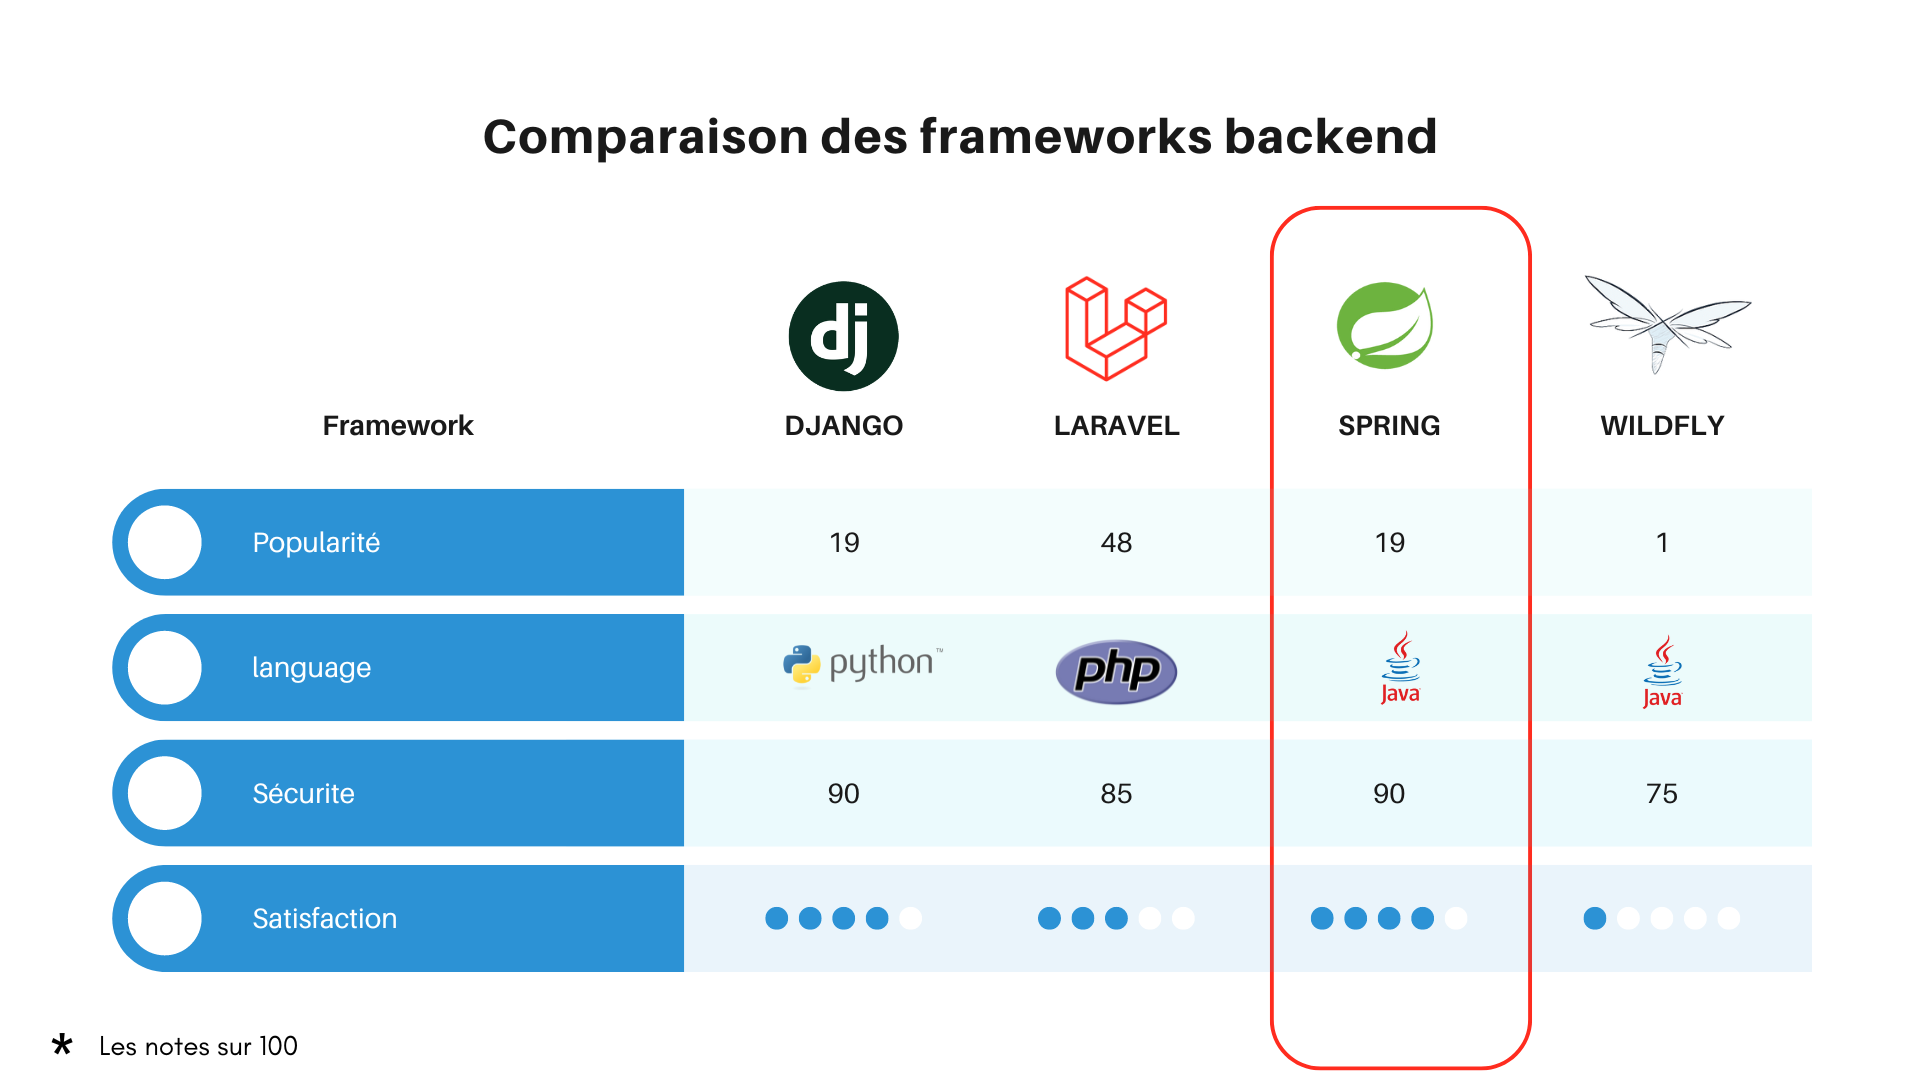
\includegraphics[width=\textwidth]{images/bechmark.png}
\caption{Diagramme de cas d'utilisation pour l'application web et le chatbot IA.}
\label{fig:bechmark}
\end{figure}



\subsection{FastAPI pour le Deploiement de Modèle de Chatbot}
% Logo de FastAPI, Docker et Modèle de Chatbot
\begin{center}

\includegraphics[height=1.5cm]{python.png}

\includegraphics[height=1.5cm]{fastapi.png}
\end{center}

FastAPI a ete choisi pour le developpement des services d'API REST en raison de sa rapidite, de sa simplicite et de sa prise en charge automatique de la documentation interactive basee sur les specifications OpenAPI (anciennement Swagger). FastAPI permet de creer des applications web Python hautement performantes, avec une validation automatique des donnees, une generation automatique de la documentation et une prise en charge asynchrone.


De plus, FastAPI est utilise specifiquement pour deployer le modèle du chatbot. Grâce à sa prise en charge asynchrone et à sa haute performance, FastAPI offre un moyen efficace de fournir des interfaces d'API pour l'interaction avec le modèle de chatbot, permettant ainsi une integration facile avec d'autres services et applications.






\subsection{Keycloak pour la Gestion des Identites et des Accès}
% Logo de Keycloak
\begin{center}

\includegraphics[height=2cm]{images/keycloak.png}
\end{center}

Keycloak est une solution essentielle pour la gestion des identites et des accès dans les architectures microservices. Cette plateforme open-source offre une gestion integree de l'authentification et de l'autorisation des utilisateurs, ce qui en fait un choix privilegie pour securiser les applications distribuees.

Dans une architecture microservices, où les services sont deployes et executes de manière independante, la gestion des identites et des accès devient une tâche complexe. Keycloak permet de centraliser cette gestion en fournissant un système robuste de gestion des utilisateurs, des rôles et des permissions. Cela simplifie grandement le processus d'integration de la securite dans les microservices, en offrant une solution unifiee pour l'authentification et l'autorisation des utilisateurs.

L'un des avantages majeurs de Keycloak est sa capacite à fournir une authentification securisee, en supportant des protocoles standard tels que OAuth 2.0 et OpenID Connect. Cela permet aux applications de beneficier d'une authentification multi-facteurs, de la gestion des sessions utilisateur, et de la gestion des tokens d'accès, garantissant ainsi la securite des donnees et des transactions.

En outre, Keycloak offre des fonctionnalites avancees telles que la gestion des flux de travail d'approbation, la gestion des sessions utilisateur et la gestion des politiques d'accès. Ces fonctionnalites permettent de mettre en place des strategies de securite flexibles et personnalisees, adaptees aux besoins specifiques de chaque application.

En resume, Keycloak joue un rôle crucial dans les architectures microservices en fournissant une solution complète et securisee pour la gestion des identites et des accès. Son integration simplifiee, ses fonctionnalites avancees et son support des standards de l'industrie en font un choix ideal pour garantir la securite des applications distribuees.


\subsection{Git et GitHub pour la Gestion de Version et la Collaboration}
% Logos de Git et GitHub
\begin{center}

\includegraphics[height=1.5cm]{git.png}

\includegraphics[height=1.5cm]{github.png}
\end{center}

Git est un système de contrôle de version distribue largement utilise dans l'industrie du developpement logiciel. Il offre un moyen efficace de suivre les modifications apportees au code source et de collaborer avec d'autres developpeurs sur un projet. Git permet de creer des branches pour travailler sur des fonctionnalites isolees, fusionner les modifications en toute securite et revenir à des versions anterieures du code si necessaire.

GitHub, quant à lui, est une plateforme d'hebergement de code basee sur Git, offrant des fonctionnalites supplementaires pour la collaboration et la gestion de projet. Sur GitHub, les developpeurs peuvent heberger leurs depôts Git, suivre les problèmes, gerer les demandes de tirage (pull requests), et automatiser les workflows de developpement à l'aide de GitHub Actions.

L'utilisation de Git et GitHub dans le processus de developpement permet une collaboration efficace entre les membres de l'equipe, même dans des environnements distribues. Les fonctionnalites de suivi des modifications, de gestion des branches et de gestion de projet offertes par Git et GitHub facilitent la coordination des efforts et la mise en œuvre des meilleures pratiques de developpement logiciel telles que le developpement collaboratif et la revue de code.

En resume, Git et GitHub jouent un rôle essentiel dans le processus de developpement en offrant un moyen efficace de gerer la version du code source, de collaborer avec d'autres developpeurs et de coordonner les efforts au sein de l'equipe de developpement.


\subsection{Jenkins pour CI/CD}
% Logo de Jenkins
\begin{center}

\includegraphics[height=1.5cm]{jenkins.png}
\end{center}

Jenkins a ete integre dans le processus de developpement pour automatiser les tâches de CI/CD (Continuous Integration/Continuous Delivery). En tant qu'outil open source largement utilise, Jenkins offre une plateforme flexible et extensible pour automatiser le processus de construction, de test et de deploiement des applications.

L'un des principaux avantages de Jenkins est sa grande flexibilite et sa capacite à s'integrer avec une variete d'outils et de technologies. Il prend en charge une large gamme de plugins qui permettent d'etendre ses fonctionnalites pour repondre aux besoins specifiques du projet. Jenkins permet de configurer des pipelines de deploiement automatises, qui orchestrent les differentes etapes du processus de developpement, de la compilation du code à son deploiement sur les environnements de production.

Compare à d'autres outils de CI/CD tels que GitLab CI/CD ou Travis CI, Jenkins se distingue par sa flexibilite et sa large adoption dans l'industrie. Son interface utilisateur intuitive et ses nombreuses fonctionnalites en font un choix populaire pour les equipes de developpement cherchant à automatiser leurs workflows de developpement logiciel.

En resume, Jenkins est un outil puissant pour la mise en œuvre de pipelines CI/CD, offrant une automatisation flexible et robuste des processus de developpement, de la compilation à la livraison continue des applications.


\subsection{PostgreSQL pour la Gestion de Base de Donnees}
% Logo de PostgreSQL
\begin{center}

\includegraphics[height=1.5cm]{postgres.png}
\end{center}

PostgreSQL est un système de gestion de base de donnees relationnelle open-source repute pour sa fiabilite, sa robustesse et sa conformite aux normes SQL. Il offre un large eventail de fonctionnalites avancees, telles que le support du langage de programmation PL/pgSQL, des index avances, des procedures stockees, des transactions ACID-compliant, et bien plus encore.

Dans le contexte des architectures microservices, PostgreSQL est souvent choisi comme système de gestion de base de donnees en raison de sa capacite à gerer des charges de travail elevees, à evoluer facilement avec la croissance de l'application, et à garantir la coherence des donnees dans un environnement distribue. PostgreSQL offre egalement un support complet pour les fonctionnalites de replication, de partitionnement, de sauvegarde et de restauration, ce qui en fait un choix ideal pour les applications necessitant une gestion avancee des donnees.

De plus, PostgreSQL est largement pris en charge par les fournisseurs de services cloud, ce qui facilite son deploiement et son integration dans des environnements cloud-native. Les services de base de donnees geres, tels que Amazon RDS pour PostgreSQL et Google Cloud SQL, simplifient la gestion operationnelle de PostgreSQL en automatisant les tâches de sauvegarde, de mise à l'echelle et de maintenance.

En resume, PostgreSQL est un choix solide pour la gestion de base de donnees dans les architectures microservices, offrant une combinaison de performances elevees, de fiabilite et de fonctionnalites avancees pour repondre aux besoins complexes des applications modernes.



\subsection{IntelliJ IDEA et VS Code pour le Developpement d'Applications}
% Logos de IntelliJ IDEA et Visual Studio Code
\begin{center}

\includegraphics[height=1.5cm]{intellij.png}

\includegraphics[height=1.5cm]{vscode.jpg}
\end{center}

IntelliJ IDEA et Visual Studio Code sont deux IDE populaires utilises dans le processus de developpement pour la creation d'applications logicielles. Chacun offre un ensemble unique de fonctionnalites et d'outils qui peuvent être adaptes aux besoins specifiques des developpeurs et des projets.

IntelliJ IDEA, developpe par JetBrains, est repute pour sa puissance et sa richesse en fonctionnalites. Il offre un support complet pour de nombreux langages de programmation, notamment Java, Kotlin, Python, JavaScript, et bien d'autres. IntelliJ IDEA propose des fonctionnalites avancees telles que la completion automatique du code, la refactoring intelligent, le debogage avance, et l'integration avec des outils de gestion de version comme Git. Il offre egalement une integration etroite avec d'autres produits JetBrains, tels que IntelliJ IDEA Ultimate pour le developpement Java EE et Android.

Visual Studio Code, quant à lui, est un editeur de code leger et polyvalent developpe par Microsoft. Il offre une interface utilisateur moderne, une extensibilite remarquable grâce à un ecosystème de plugins volumineux, et une prise en charge native de nombreux langages de programmation et frameworks. Visual Studio Code est particulièrement apprecie pour son integration avec des outils de developpement web tels que Node.js, Angular, React et TypeScript, ainsi que pour ses fonctionnalites avancees de debogage et de gestion de version.

L'utilisation d'IntelliJ IDEA et de Visual Studio Code dans le processus de developpement offre une flexibilite et une productivite accrues aux developpeurs. Ces IDE offrent un ensemble complet d'outils pour la creation, la compilation, le debogage et le deploiement d'applications logicielles, tout en fournissant une experience utilisateur intuitive et personnalisable.

En resume, IntelliJ IDEA et Visual Studio Code sont deux IDE puissants et polyvalents largement utilises dans l'industrie du developpement logiciel, offrant des fonctionnalites avancees et une productivite accrue pour les developpeurs.


\subsection{Autres Technologies}

\begin{itemize}
    \item  
\includegraphics[height=1.5cm]{images/docker.png} \hspace{5pt} \textbf{Docker}: 
    Docker a ete utilise pour la containerisation des applications. Il permet de deployer facilement des environnements de developpement, de test et de production homogènes. La containerisation assure que les applications fonctionnent de manière coherente dans differents environnements.

    \item 
\includegraphics[height=1.5cm]{images/mongo.png} \hspace{5pt} \textbf{MongoDB}  : 
    MongoDB est une base de donnees NoSQL utilisee pour stocker les donnees non structurees du chatbot. Elle offre une grande flexibilite dans la gestion des donnees, ce qui est ideal pour les applications necessitant une structure de donnees dynamique et evolutive.

    \item 
\includegraphics[height=1.5cm]{images/postgres.png} \hspace{5pt} \textbf{PostgreSQL}  : 
    PostgreSQL est utilise pour la gestion des donnees relationnelles. Cette base de donnees relationnelle open-source est reputee pour sa robustesse, sa performance et sa conformite aux standards SQL, ce qui en fait un choix ideal pour les applications necessitant une forte integrite des donnees.

    \item 
\includegraphics[height=1.5cm]{images/redis.png} \hspace{5pt} \textbf{Redis} : 
    Redis est utilise pour la gestion du cache pour ameliorer les performances des applications. Ce magasin cle-valeur en memoire permet de reduire la latence des requêtes et d'ameliorer le temps de reponse global du système.

    \item 
\includegraphics[height=1.5cm]{images/kubernetes.png} \hspace{5pt} \textbf{Kubernetes} : 
    Kubernetes a ete utilise pour l'orchestration des conteneurs Docker. Il permet de deployer, de gerer et de mettre à l'echelle automatiquement les applications containerisees, assurant ainsi une haute disponibilite et une gestion efficace des ressources.

    \item 
\includegraphics[height=1.5cm]{images/jwt.png} \hspace{5pt} \textbf{JWT (JSON Web Token)}  : 
    JWT est utilise pour l'authentification securisee des utilisateurs. Les tokens JWT permettent de securiser les echanges entre les differentes parties de l'application en garantissant l'integrite et l'authenticite des informations transmises.


\item 
\includegraphics[height=1.5cm]{images/langchain.jpeg} \hspace{5pt} \textbf{LangChain}  : 
LangChain est utilise pour la gestion des chaînes de langage naturel dans le chatbot. Il permet de structurer et de manipuler les flux conversationnels, offrant une meilleure experience utilisateur en facilitant la comprehension et la generation de textes par le chatbot.

\item 
\includegraphics[height=1.5cm]{images/llm.png} \hspace{5pt} \textbf{LLM (Large Language Model)} : 
Les Large Language Models (LLM) sont utilises pour l'intelligence artificielle du chatbot. Ces modèles puissants, entraînes sur des ensembles de donnees massifs, permettent au chatbot de comprendre et de generer un langage naturel de haute qualite, ameliorant ainsi la pertinence et la precision des reponses fournies aux utilisateurs.

\item 
\includegraphics[height=1.5cm]{images/kafka.png} \hspace{5pt} \textbf{Kafka}  : 
Kafka est utilise pour la gestion de la communication entre les microservices. Ce système de messagerie distribuee permet de transmettre des flux de donnees en temps reel, assurant une communication fiable et evolutive entre les differents composants de l'application. Kafka est ideal pour gerer les charges massives de donnees et les operations asynchrones.

\end{itemize}

\chapter{MISE EN ŒUVRE DU SPRINT 1 :Developpement et Deploiement du Chatbot}


\section{Introduction}
Dans le cadre du sprint 1, l'equipe s'est concentree sur le developpement initial du chatbot ainsi que sur son deploiement pour les premiers tests et evaluations. Voici un aperçu des activites realisees durant cette periode :


\section{Le back log su sprint 1}
\subsubsection{User Story 1.1 : Configuration Initiale du Chatbot}

\begin{itemize}
    \item \textbf{En tant que} developpeur
    \item \textbf{Je veux} configurer le cadre initial du chatbot
    \item \textbf{Afin de} disposer d’une base solide sur laquelle construire
    \item \textbf{Critères d’acceptation} :
    \begin{itemize}
        \item Le cadre du chatbot est configure et integre dans la plateforme.
        \item Les capacites conversationnelles de base sont mises en place.
    \end{itemize}
\end{itemize}

\subsubsection{User Story 1.2 : Base de Connaissances du Chatbot}

\begin{itemize}
    \item \textbf{En tant qu'} utilisateur
    \item \textbf{Je veux} poser des questions au chatbot sur Code212
    \item \textbf{Afin de} recevoir des informations specifiques sur l’ecole
    \item \textbf{Critères d’acceptation} :
    \begin{itemize}
        \item Le chatbot peut repondre avec precision aux questions sur Code212.
        \item La base de connaissances comprend des informations sur les cours, les evenements et les examens de certification.
    \end{itemize}
\end{itemize}

\section{Benchmarking et justification des technologies utilisees en Sprint 1}

Le Sprint 1 a ete consacre au developpement et au deploiement du chatbot en utilisant Llama 2, LangChain et FastAPI.

\begin{itemize}
\item Performances superieures
\item Flexibilite des domaines de connaissances
\end{itemize}

 LangChain

LangChain a ete choisi comme interface de dialogue pour sa flexibilite et sa capacite à gerer des conversations complexes. Il permet de creer des dialogues dynamiques et personnalises en fonction du contexte de la conversation.

\begin{itemize}
\item Flexibilite des dialogues
\item Gestion des conversations complexes
\item Dialogues dynamiques et personnalises
\end{itemize}

FastAPI

FastAPI a ete choisi comme framework web pour sa simplicite, sa performance et sa facilite d'utilisation. Il permet de creer des API RESTful rapidement et efficacement.

\begin{itemize}
\item Simplicite
\item Performance
\item Facilite d'utilisation
\item Creation rapide et efficace d'API RESTful
\end{itemize}

 Justification des choix

Le choix de Llama 2 et LangChain repond à deux exigences importantes du client :

* **Flexibilite des ressources:** Llama 2 permet de changer facilement les ressources du chatbot en fonction des besoins du client.

\begin{itemize}
\item Changement facile des ressources du chatbot
\end{itemize}

* **Fine-tuning efficace:** LangChain permet de realiser un fine-tuning rapide et efficace du chatbot, sans necessiter de materiel puissant.

\begin{itemize}
\item Fine-tuning rapide et efficace
\item Pas de materiel puissant necessaire
\end{itemize}

 Conclusion

Le choix des technologies pour le Sprint 1 a ete guide par la recherche de solutions performantes, flexibles et adaptees aux besoins du client. Llama 2, LangChain et FastAPI constituent une combinaison puissante qui permet de creer un chatbot performant et evolutif.


\section{Analyse et Conception}
\subsection{Description textuel}

\begin{itemize}
    \item \textbf{Analyse des besoins :} L'equipe a mene une analyse approfondie des besoins des utilisateurs finaux pour definir les fonctionnalites initiales du chatbot. Cela a inclus l'identification des cas d'utilisation principaux, des scenarios de conversation et des integrations système necessaires.
    
    \item \textbf{Conception de l'architecture :} Sur la base des besoins identifies, l'architecture du chatbot a ete conçue, en determinant les composants principaux, les flux de donnees et les integrations externes requises. L'objectif etait de garantir la scalabilite, la flexibilite et la facilite de maintenance du chatbot.
    
    \item \textbf{Developpement initial :} Le developpement initial du chatbot a debute, en se concentrant sur la mise en place de l'infrastructure de base, la creation des modèles de conversation, et l'integration avec les outils de traitement du langage naturel (NLP) et les sources de donnees.
    
    \item \textbf{Tests unitaires :} Des tests unitaires ont ete mis en place pour valider le bon fonctionnement des differentes fonctionnalites du chatbot. Cela a permis de detecter et de corriger rapidement les eventuels bogues ou problèmes de fonctionnalite.
    
    \item \textbf{Deploiement initial :} Une version initiale du chatbot a ete deployee sur un environnement de test pour permettre aux membres de l'equipe et aux parties prenantes de l'evaluer et de fournir des retours d'experience. Cela a egalement permis de commencer à collecter des donnees d'utilisation reelles pour ameliorer la performance et la pertinence du chatbot.
\end{itemize}

\subsection{Diagramme de cas d'utilisation du sprint 1}
\begin{figure}[H]
\centering
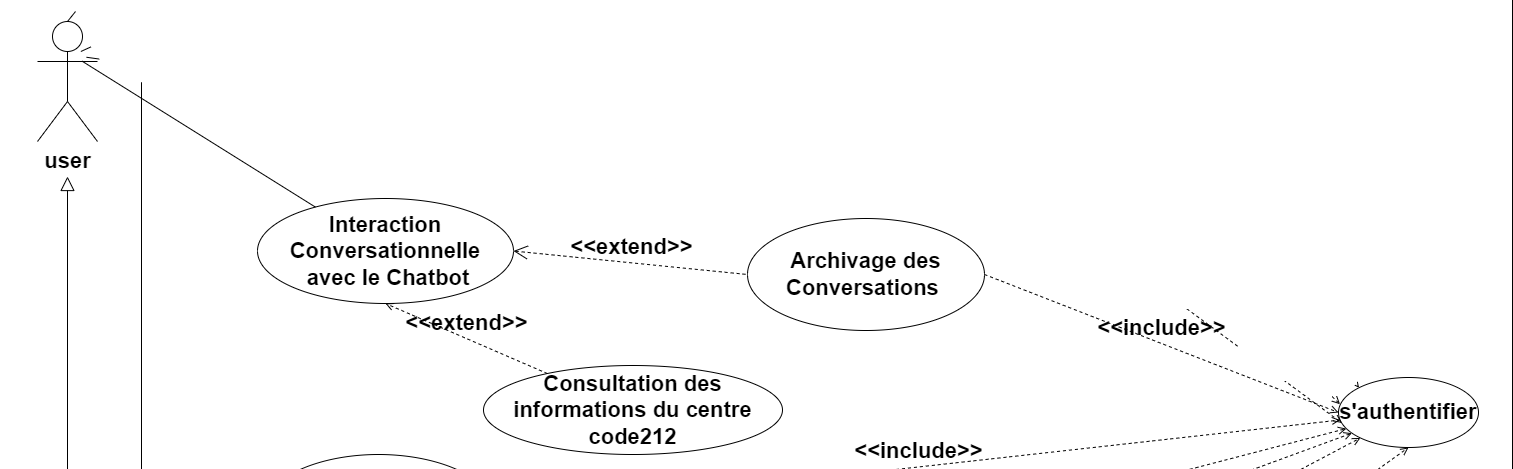
\includegraphics[width=\textwidth]{sprint1-usecase.png}
\caption{Diagramme de cas d'utilisation du sprint 1}
\label{fig:sprint1_usecase}
\end{figure}


\subsection{Diagramme de classe du sprint 1}
\begin{figure}[H]
\centering
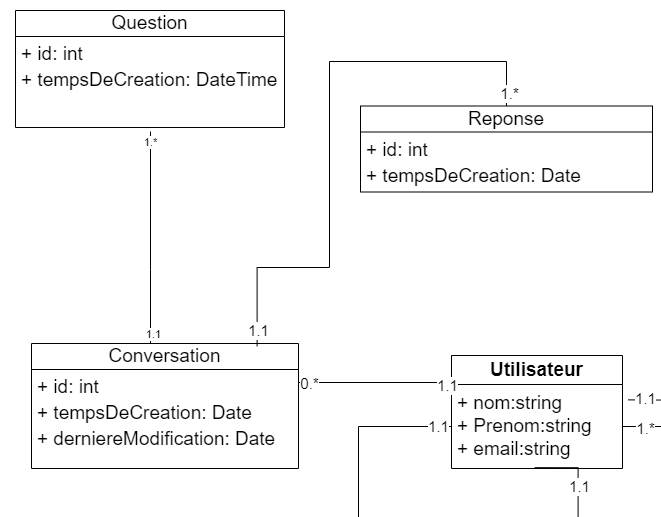
\includegraphics[width=\textwidth]{sprint1-class.png}
\caption{Diagramme de classe du sprint 1}
\label{fig:sprint1_class}
\end{figure}

\subsection{Retrieval-Augmented Generation :}
\clearpage
\begin{figure}[H]
\centering
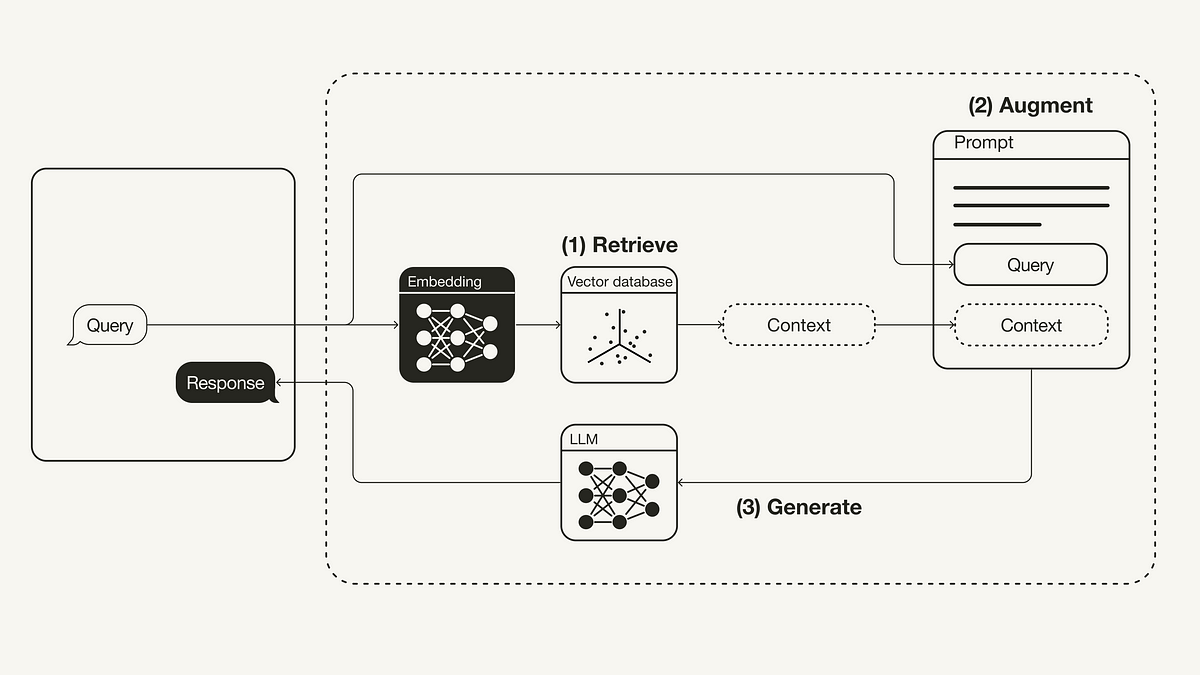
\includegraphics[width=\textwidth]{images/rag.png} 
\caption{Diagramme de l'architecture RAG}
\label{fig:rag}
\end{figure}
RAG est un modèle NLP qui ameliore la generation de texte en integrant des informations recuperees à partir d'une base de donnees ou d'un corpus de documents externes




\subsection{Diagramme de sequence du sprint 1}
\begin{figure}[H]
\centering
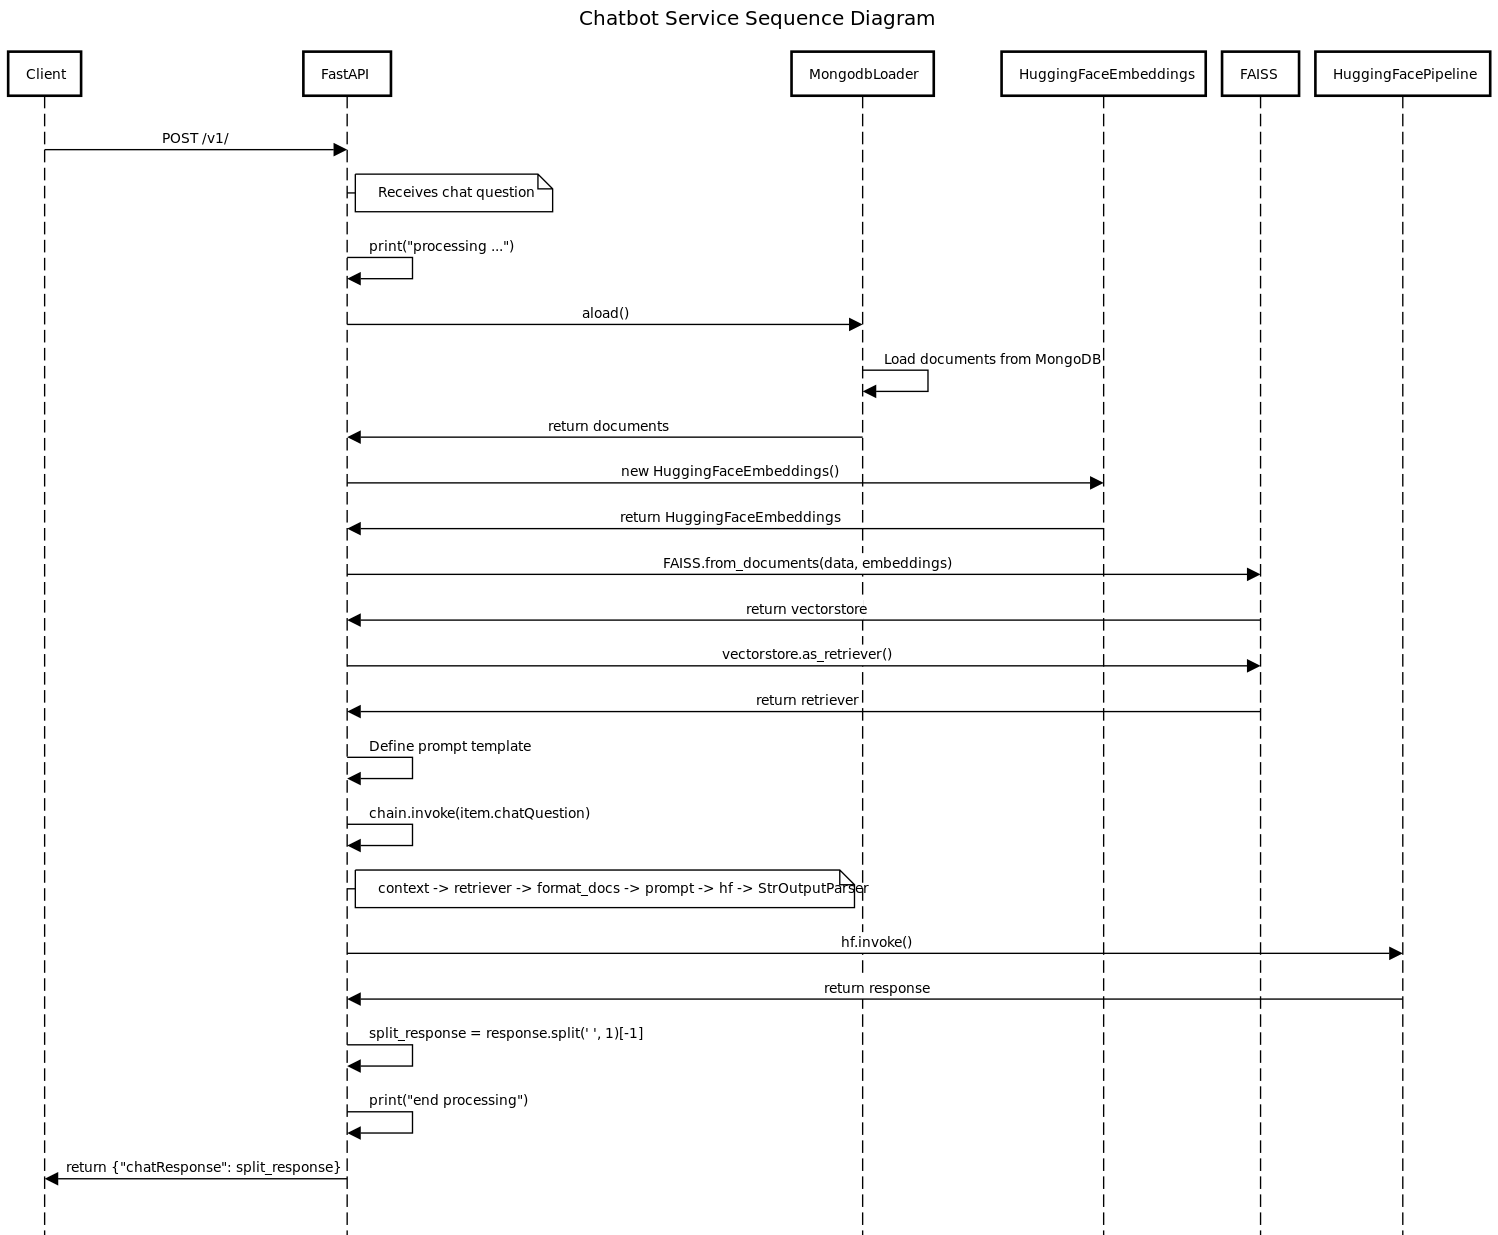
\includegraphics[width=1.2\textwidth]{chatbot-seq.png}
\caption{Diagramme de sequence du sprint 1}
\label{fig:sprint1_seq}
\end{figure}

\section{Realisation du sprint 1}

% Espace pour inclure des images de chat
\begin{center}
    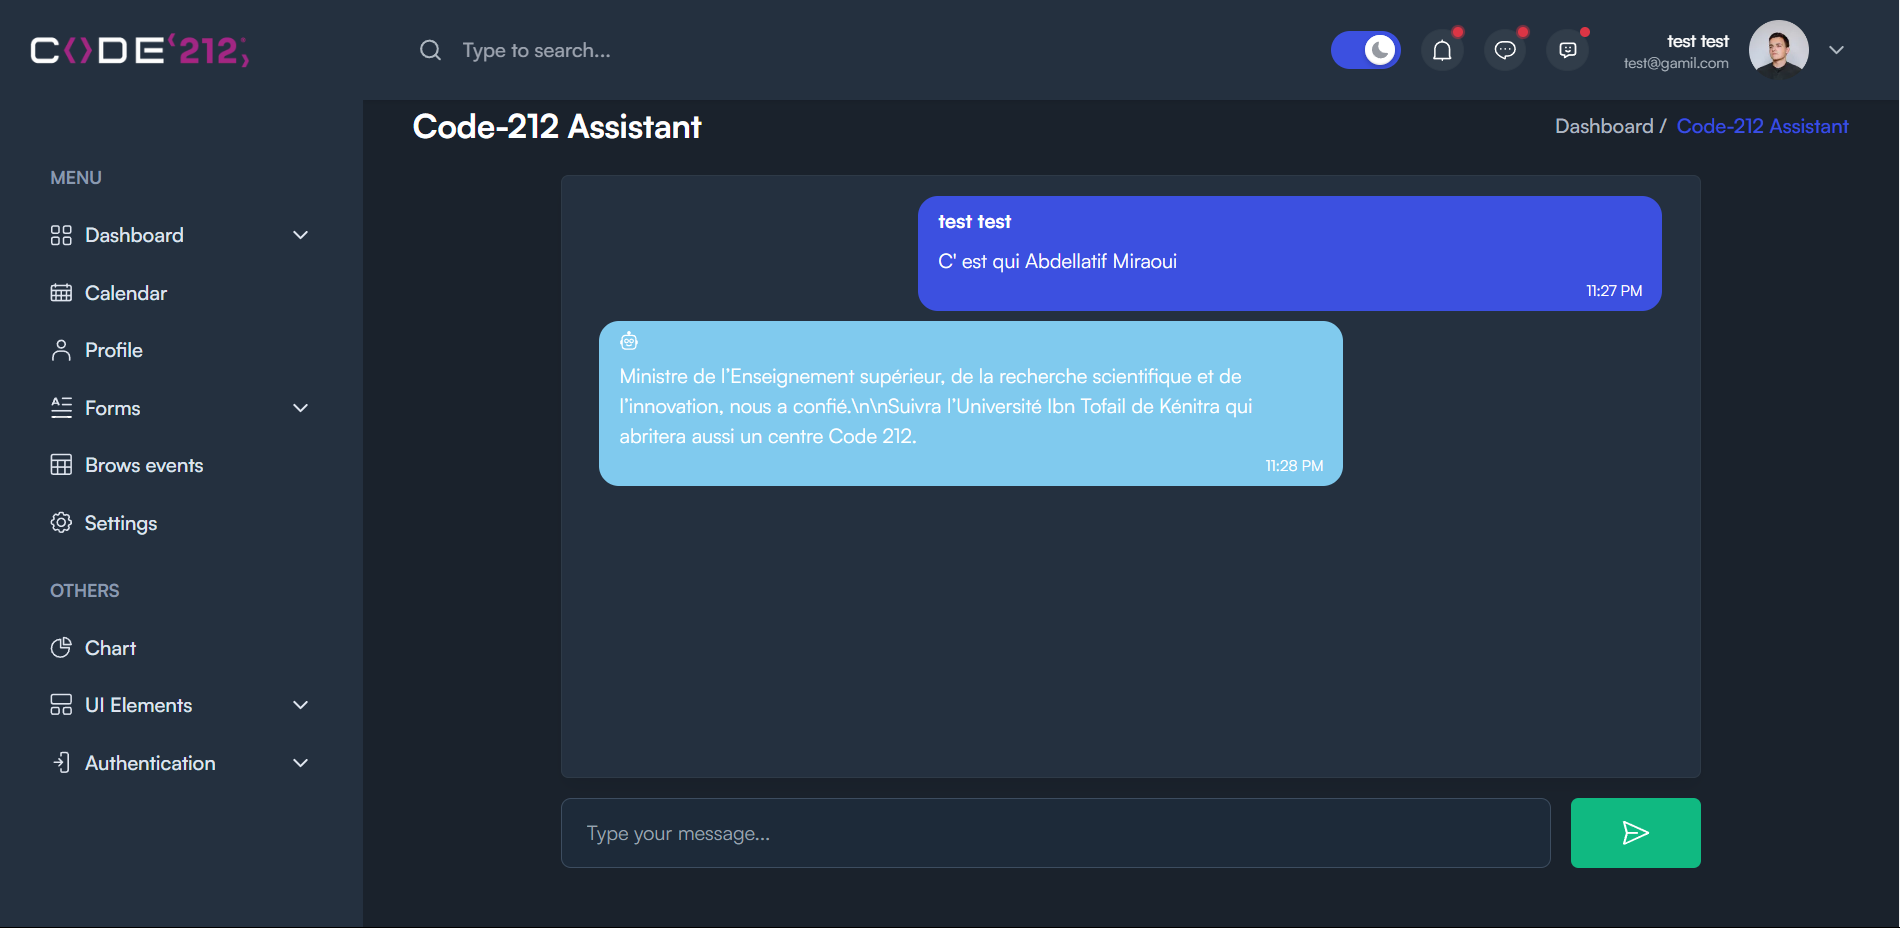
\includegraphics[width=1\textwidth]{chat1.png}
    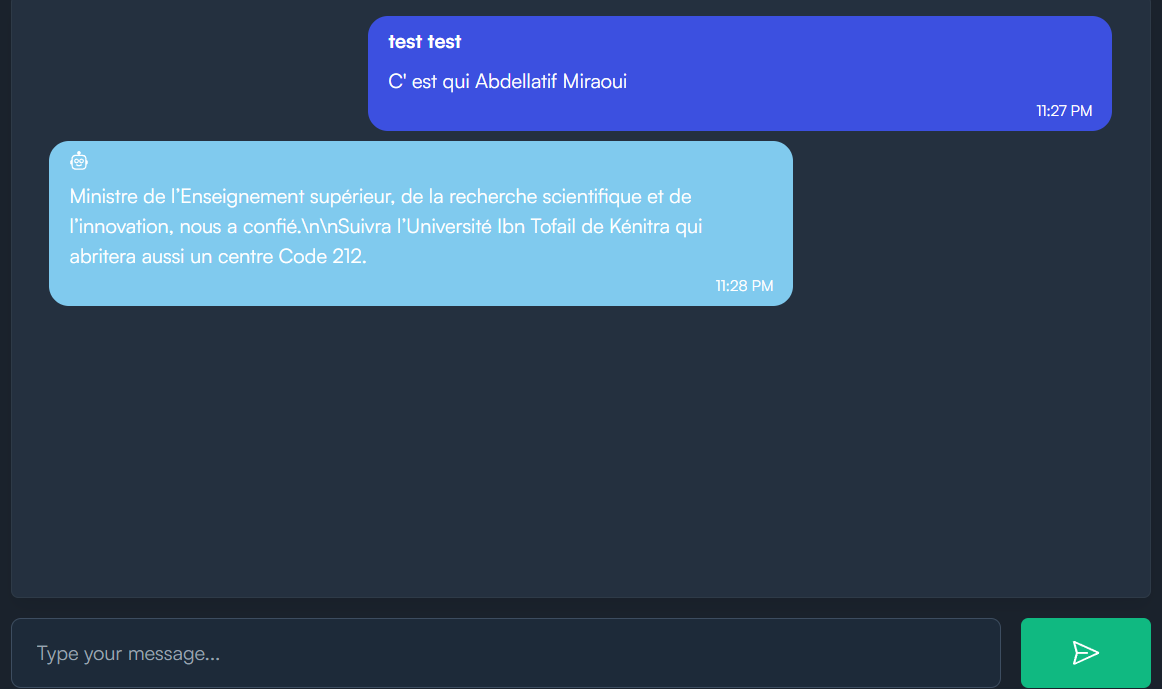
\includegraphics[width=1\textwidth]{chat2.png}
\end{center}

L' images ci-dessus montre un exemple de conversation avec le chatbot lors des premiers tests. Ces captures d'ecran illustrent la convivialite de l'interface utilisateur et la capacite du chatbot à repondre efficacement aux requêtes des utilisateurs.


Pour le developpement du chatbot, le modèle Llama 2 a ete utilise comme base de l'infrastructure de traitement du langage naturel. Llama 2 est un modèle pre-entraîne puissant qui offre des capacites avancees de generation de texte et d'analyse de langage naturel, ce qui en fait un choix ideal pour la creation d'un chatbot intelligent et reactif.

Le sprint 1 a pose les bases du developpement du chatbot, en mettant en place les fondations necessaires pour son evolution future. Les retours d'experience recueillis lors de cette phase ont ete precieux pour orienter les prochains travaux et assurer le succès du projet.




\chapter{MISE EN ŒUVRE DU SPRINT 2: Authentification et mise a jour de la base de donnees par l’administrateur}
\section{Introduction}

Dans le cadre du sprint 2, l'equipe s'est concentree sur authentification et la mise à jour de la base de donnees par le gestionnaire, conformement à l'User Story 1.3. Cette fonctionnalite permet au gestionnaire d'effectuer des modifications sur les ressources du chatbot via l'application, qui est connectee à MongoDB. Voici les details de cette etape :

\section{Backlog du Sprint 2}

Le developpement de notre application de gestion de chatbot s’est structure autour d’un backlog produit bien defini, comprenant plusieurs epopees et user stories. Chaque user story a ete accompagnee de critères d’acceptation clairs pour garantir la qualite et la conformite aux attentes.

\subsection{epopee 1 : Authentification et mise à Jour de la Base de Donnees par l’Administrateur}

\textbf{Authentification se fait par Keycloak}

\textbf{User Story 1.3 : Mise à Jour de la Base de Donnees par l’Administrateur}
\begin{itemize}
    \item \textbf{En tant que :} administrateur
    \item \textbf{Je veux :} pouvoir mettre à jour la base de donnees du chatbot à tout moment
    \item \textbf{Afin de :} m’assurer que les informations sont toujours à jour
    \item \textbf{Critères d'acceptation :}
    \begin{itemize}
        \item L’administrateur peut acceder à une interface pour mettre à jour la base de donnees.
        \item Les modifications sont immediatement refletees dans les reponses du chatbot.
    \end{itemize}
\end{itemize}

\subsection{Sprint Plan}
\begin{itemize}
    \item \textbf{Sprint 2 :} Mise à jour de la base de donnees par l’administrateur (User Story 1.3), Consultation des cours disponibles (User Story 2.1)
\end{itemize}

\section{Analyse et Conception}
\subsection{Description textuel}
\begin{itemize}
    \item **Analyse des Besoins :** L'equipe a etudie les exigences de l'User Story 1.3 pour comprendre les fonctionnalites specifiques attendues par le gestionnaire. Cela comprenait la capacite de modifier les ressources du chatbot telles que les reponses predefinies, les questions frequemment posees, etc.
    
    \item **Developpement de l'Application :** Une application dediee a ete developpee, offrant une interface conviviale permettant au gestionnaire d'acceder et de modifier les ressources du chatbot directement via MongoDB. L'application a ete conçue pour être securisee et intuitive, garantissant une experience utilisateur optimale.
    
    \item **Integration avec MongoDB :** L'application a ete connectee à MongoDB pour permettre une interaction transparente avec la base de donnees. Cela a permis au gestionnaire d'acceder aux donnees du chatbot en temps reel et de les modifier selon ses besoins, sans necessiter de connaissances techniques avancees.
    
    \item **Tests et Validation :** Une serie de tests ont ete effectues pour valider la fonctionnalite de mise à jour de la base de donnees par le gestionnaire. Cela comprenait des tests d'interface utilisateur, des tests de performance et des tests de securite pour garantir le bon fonctionnement de l'application dans divers scenarios d'utilisation.
\end{itemize}

\subsection{Diagramme de cas d'utilisation de sprint 2}


\begin{figure}[H]
\centering
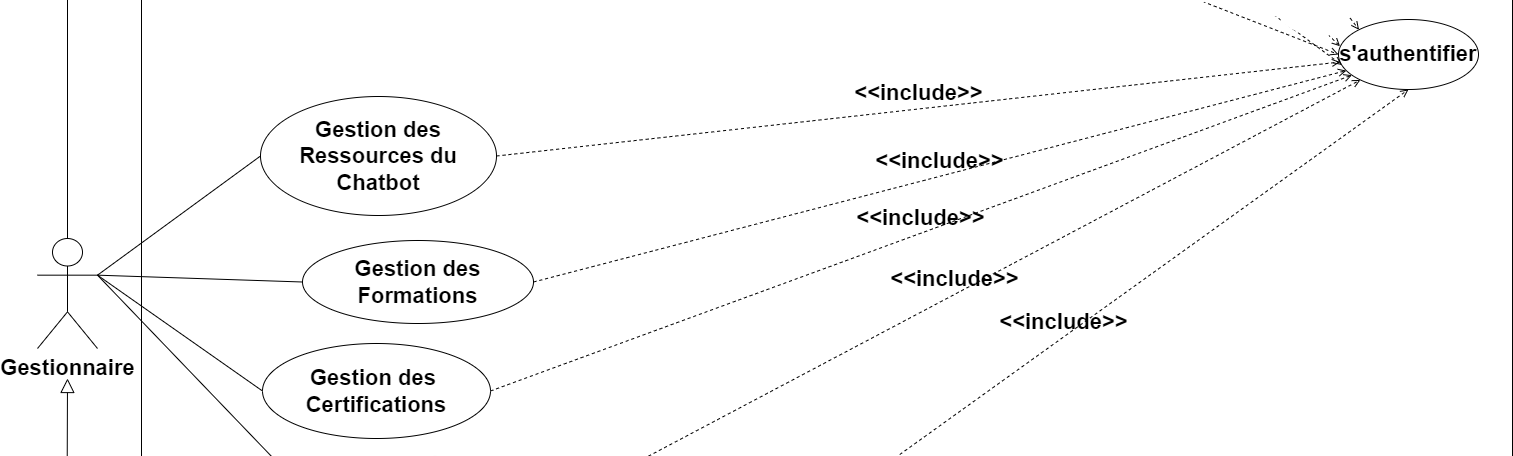
\includegraphics[width=\textwidth]{sprint2-usecase.png} 
\caption{Diagramme de cas d'utilisation de sprint 2}
\label{fig:s2_usecase}
\end{figure}

\subsection{Diagramme de classe de sprint 2}
\begin{figure}[H]
\centering
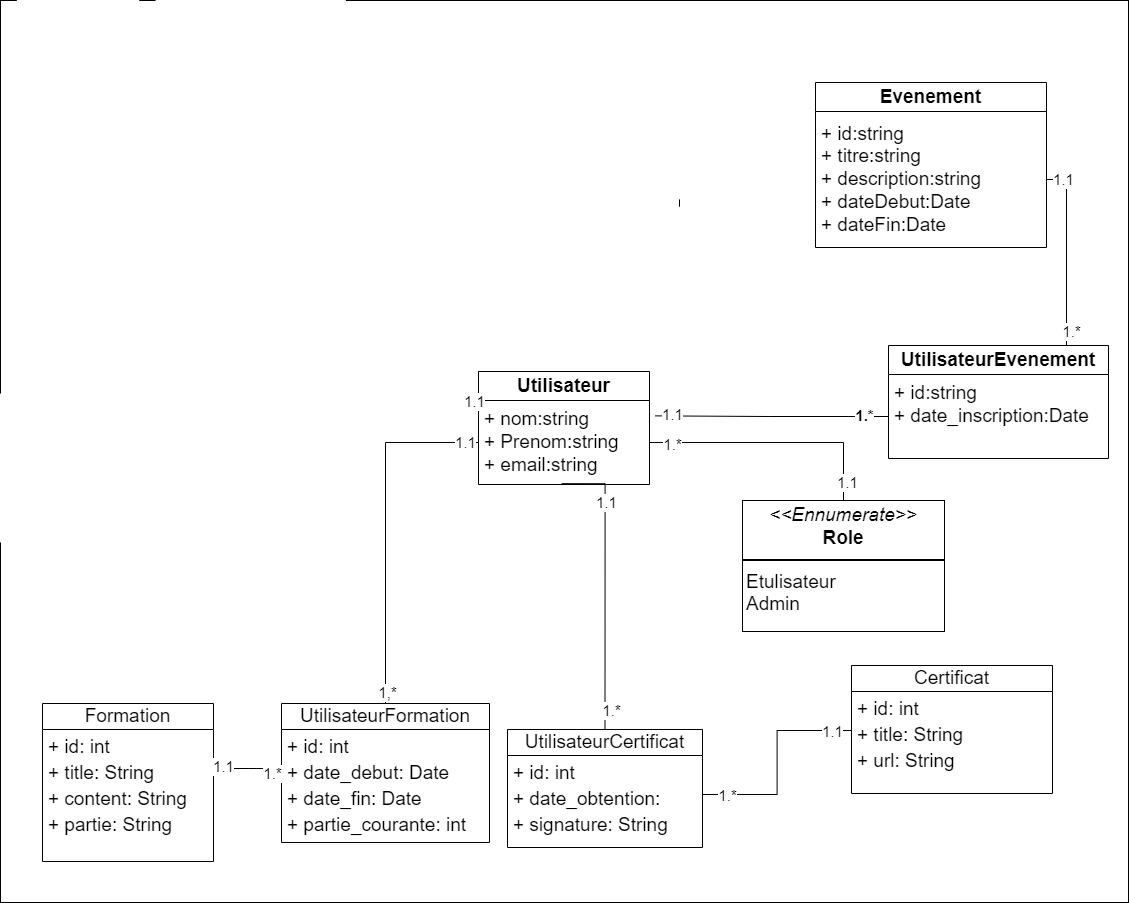
\includegraphics[width=\textwidth]{sprint2-class.png} 
\caption{Diagramme de classe de sprint 2}
\label{fig:s2_class}
\end{figure}

\subsection{Diagramme de sequence de sprint 2}


\begin{figure}[H]
\centering
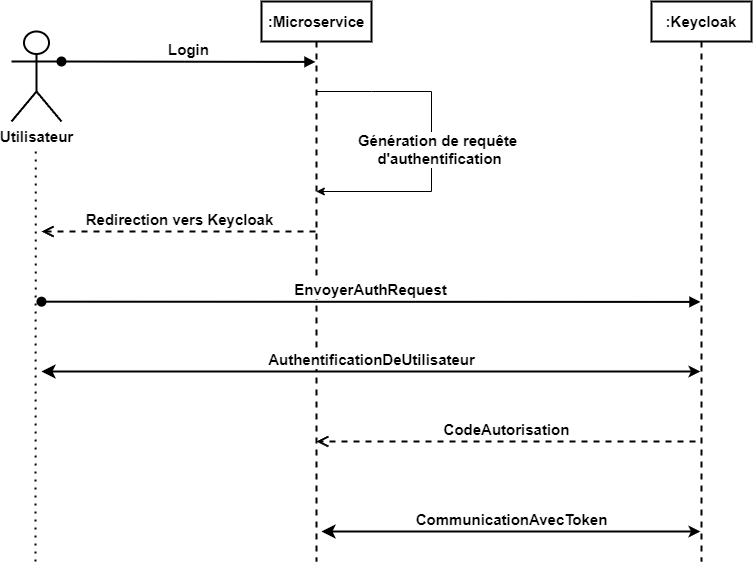
\includegraphics[width=\textwidth]{keycloak-seq.png} 
\caption{Diagramme de sequence d' authentification par Keycloak}
\label{fig:s2_auth}
\end{figure}


\begin{figure}[H]
\centering
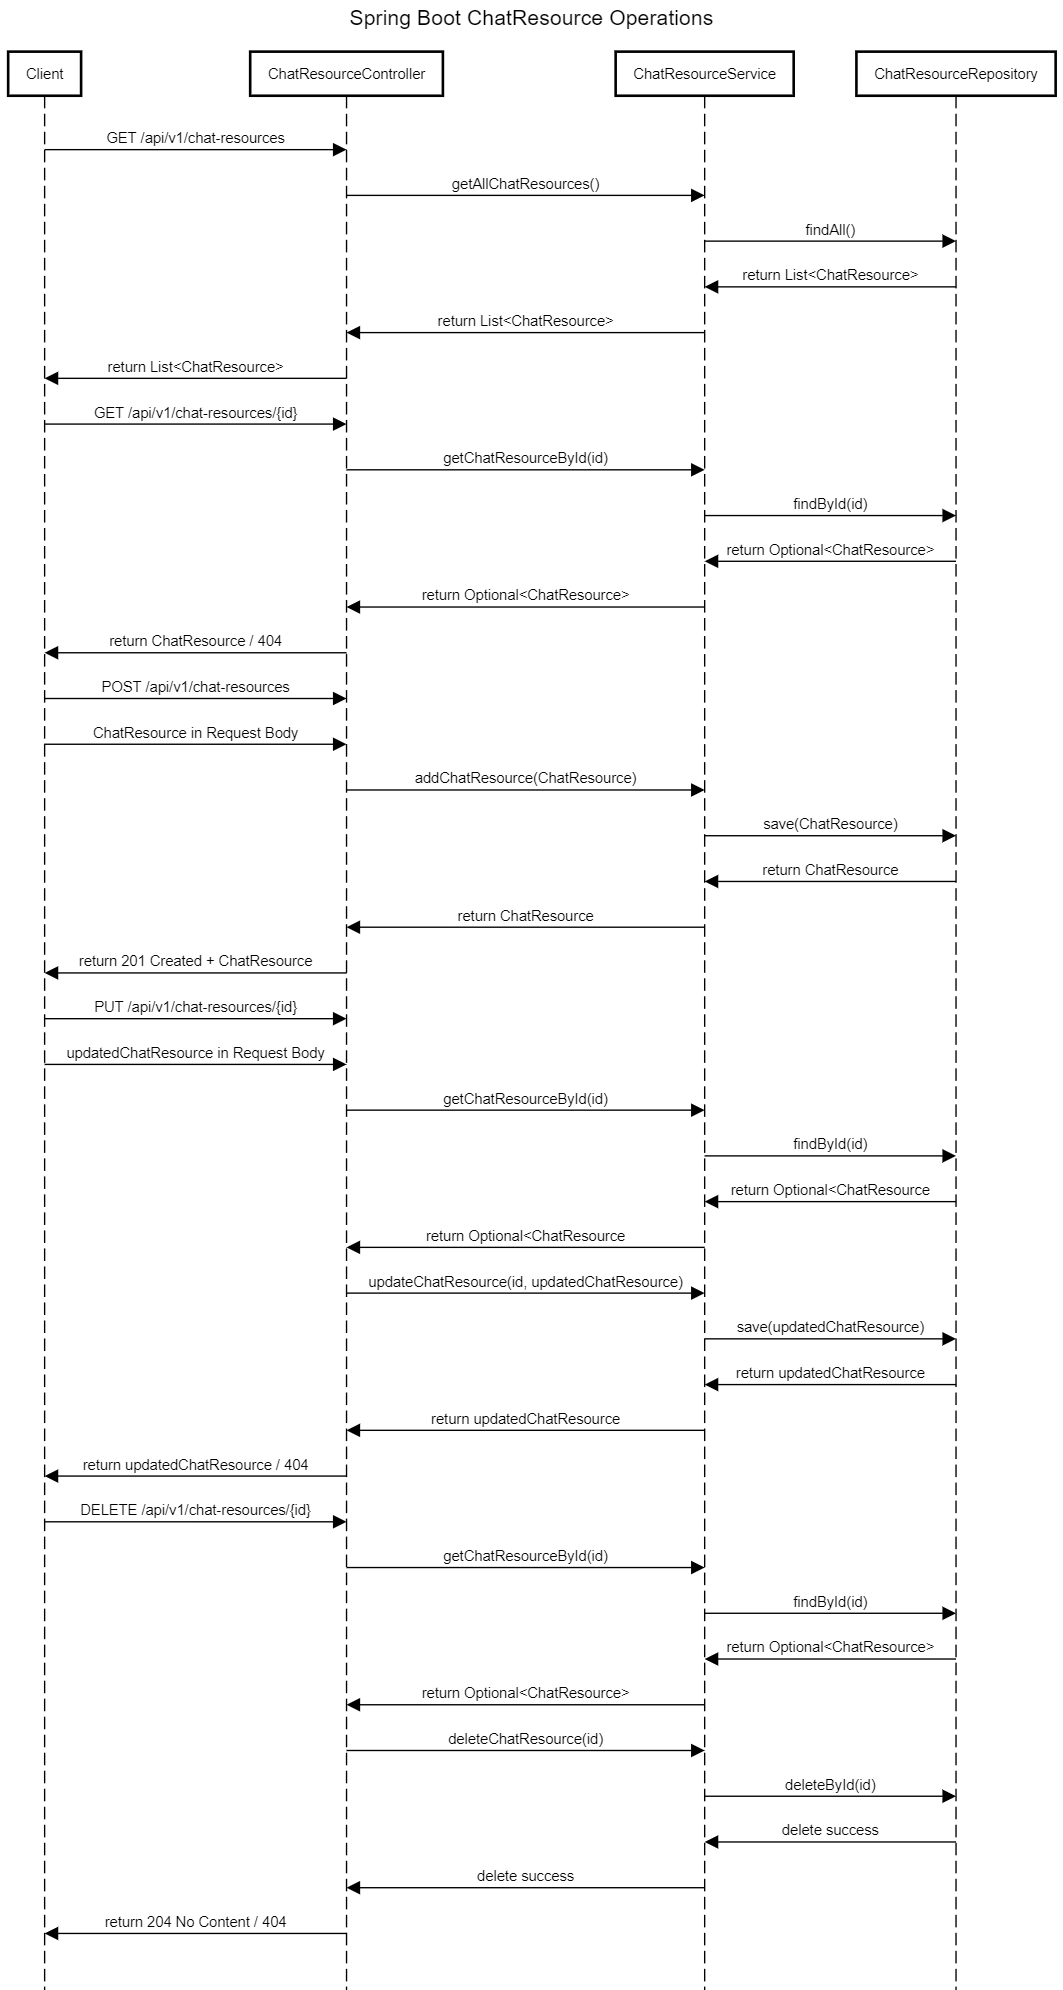
\includegraphics[width=\textwidth]{chat-res-seq.png} 
\caption{Diagramme de sequence de sprint 2}
\label{fig:chatres_seq}
\end{figure}

\section{Realisation}


\begin{figure}[H]
\centering
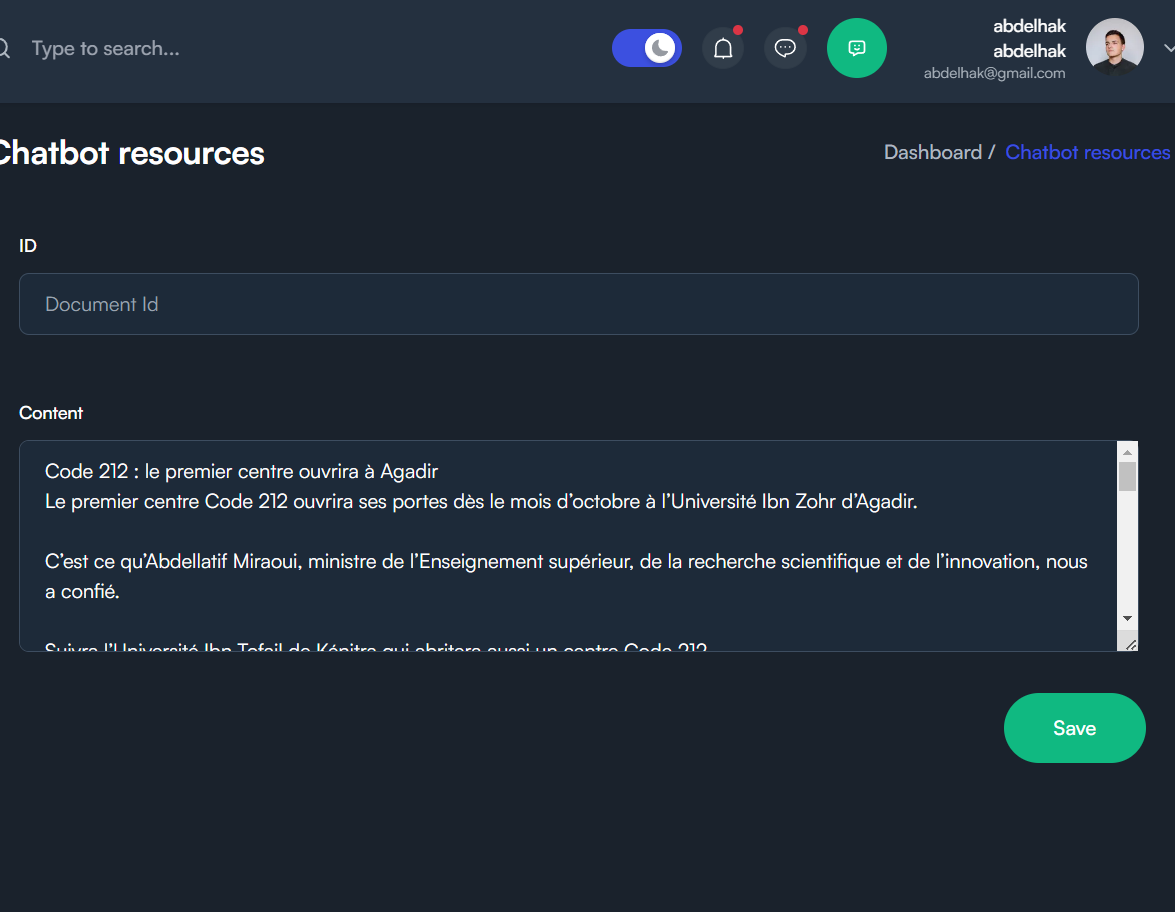
\includegraphics[width=\textwidth]{admin-doc.png} 
\caption{Capture d'ecrant d'interface qui permet au gestionnaire de modifier la base des resources du chatbot}
\label{fig:screen_chat_res}
\end{figure}

L'image ci-dessus montre un screenshot de l'application developpee pour permettre au gestionnaire de modifier les ressources du chatbot via MongoDB. Cette interface conviviale offre une vue claire et intuitive des donnees, permettant au gestionnaire d'effectuer facilement les modifications necessaires.

Le sprint 2 a permis de mettre en place une fonctionnalite essentielle pour la gestion et la maintenance du chatbot, en offrant au gestionnaire un moyen simple et efficace de mettre à jour les ressources du chatbot en temps reel.

\newpage


\chapter{MISE EN ŒUVRE DU SPRINT 3: Inscription aux cours, evenements et certificats}
\section{Introduction}

Le sprint 3 a ete consacre à la mise en œuvre de l'User Story 2.2, qui concerne l'inscription aux cours et evenements, ainsi que l'inscription aux examens de certification gratuits. Cette fonctionnalite permet aux utilisateurs de s'inscrire à des cours et evenements proposes par le Centre Code 212, ainsi qu'aux examens de certification associes. Voici les details de cette etape :

\begin{itemize}
    \item \textbf{Analyse des Besoins :} L'equipe a etudie les exigences de l'User Story 2.2 pour comprendre les fonctionnalites specifiques attendues par les utilisateurs. Cela comprenait la capacite de s'inscrire à des cours, evenements et examens de certification directement via la plateforme.
    
    \item \textbf{Developpement de l'Application :} Une fonctionnalite dediee a ete developpee, offrant une interface conviviale permettant aux utilisateurs de consulter et s'inscrire aux cours, evenements et examens de certification. L'application a ete conçue pour être securisee et intuitive, garantissant une experience utilisateur optimale.
    
    \item \textbf{Integration avec le Système de Gestion :} L'application a ete connectee au système de gestion pour permettre une interaction transparente avec les donnees de cours, evenements et examens de certification. Cela a permis aux utilisateurs d'acceder aux informations en temps reel et de s'inscrire selon leurs besoins.
    
    \item \textbf{Tests et Validation :} Une serie de tests ont ete effectues pour valider la fonctionnalite d'inscription aux cours, evenements et examens de certification. Cela comprenait des tests d'interface utilisateur, des tests de performance et des tests de securite pour garantir le bon fonctionnement de l'application dans divers scenarios d'utilisation.
\end{itemize}

\section{Backlog du Sprint 3}

Le developpement de notre application de gestion de chatbot s’est structure autour d’un backlog produit bien defini, comprenant plusieurs epopees et user stories. Chaque user story a ete accompagnee de critères d’acceptation clairs pour garantir la qualite et la conformite aux attentes.

\subsection{epopee 2 : Inscription aux Cours, evenements et Examens de Certification}

\textbf{User Story 2.2 : Inscription aux Cours et evenements}
\begin{itemize}
    \item \textbf{En tant que :} utilisateur
    \item \textbf{Je veux :} m'inscrire aux cours et evenements
    \item \textbf{Afin de :} participer à ceux-ci
    \item \textbf{Critères d'acceptation :}
    \begin{itemize}
        \item Les utilisateurs peuvent s'inscrire à des cours et des evenements via la plateforme.
        \item Un système de confirmation d'inscription est en place.
    \end{itemize}
\end{itemize}

\textbf{User Story 2.3 : Inscription aux Examens de Certification Gratuits}
\begin{itemize}
    \item \textbf{En tant que :} utilisateur
    \item \textbf{Je veux :} m'inscrire à des examens de certification gratuits
    \item \textbf{Afin de :} obtenir des certifications
    \item \textbf{Critères d'acceptation :}
    \begin{itemize}
        \item Les utilisateurs peuvent voir les examens de certification disponibles et s'y inscrire gratuitement.
        \item Un système de confirmation d'inscription aux examens est en place.
    \end{itemize}
\end{itemize}


\section{Analyse et Conception}
\subsection{Diagramme de cas d'utilisation de sprint 3}

\begin{figure}[H]
\centering
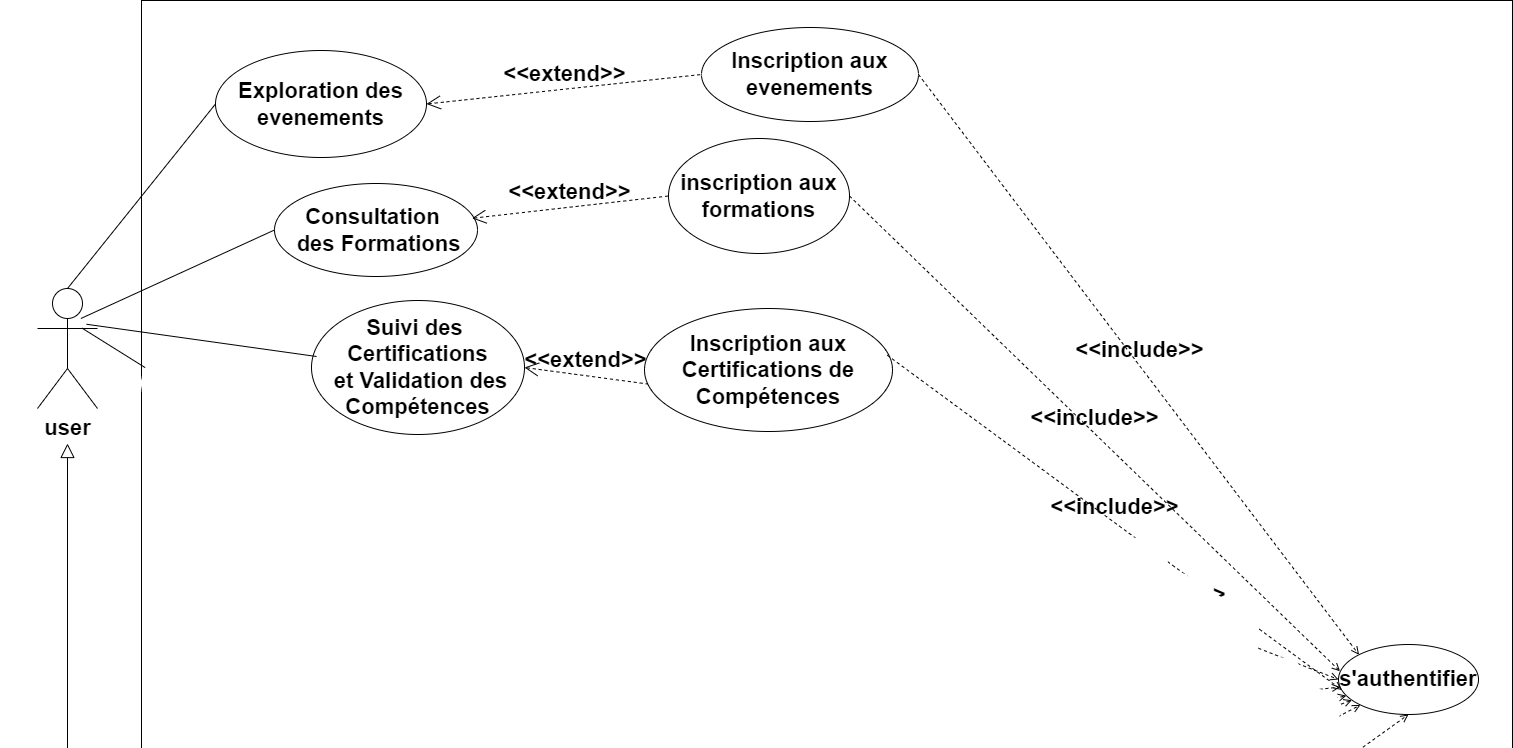
\includegraphics[width=\textwidth]{sprint3-usecase.png} 
\caption{Diagramme de cas d'utilisation de sprint 3}
\label{fig:s3-use}
\end{figure}

\subsection{Diagramme de classe de sprint 3}

\begin{figure}[H]
\centering
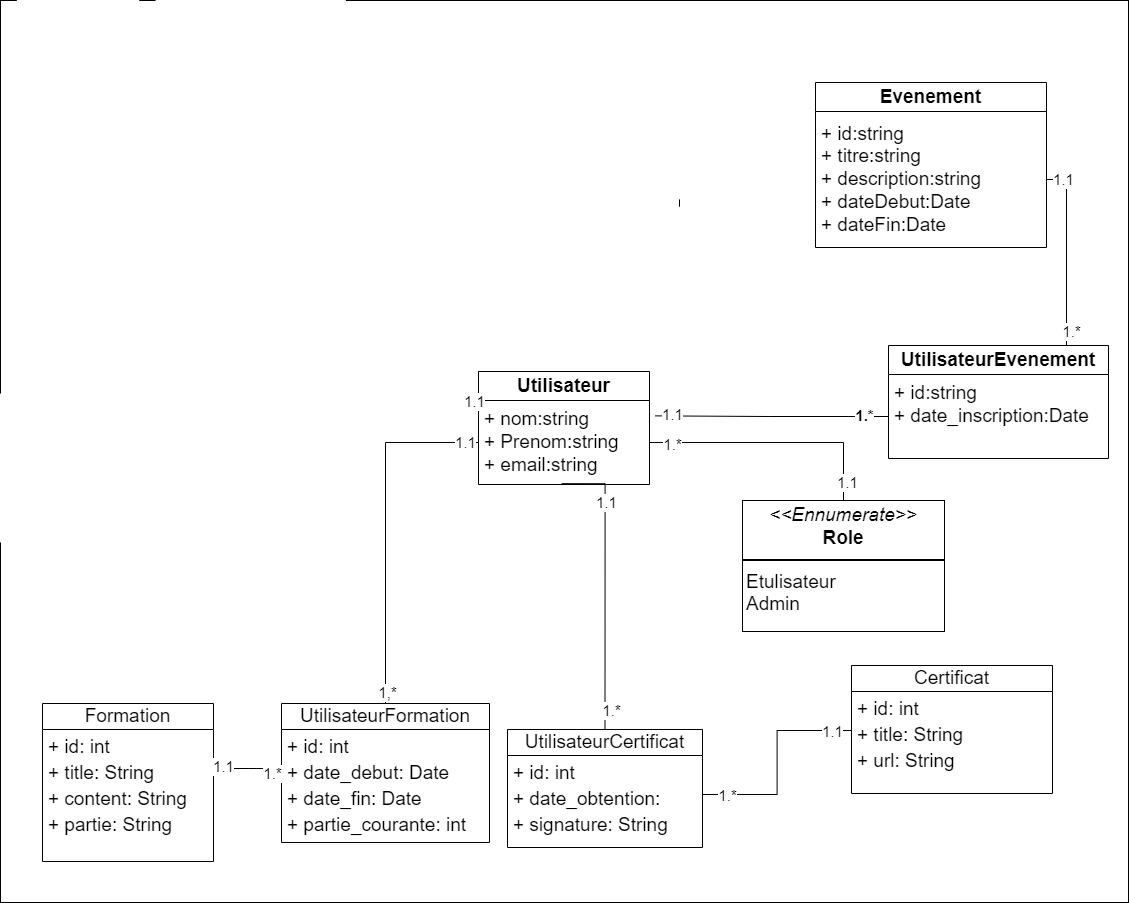
\includegraphics[width=\textwidth]{sprint2-class.png} 
\caption{Diagramme de classe de sprint 3}
\label{fig:s3_class}
\end{figure}

\subsection{Diagramme de Sequence de sprint 3}
\clearpage
\begin{figure}
\centering
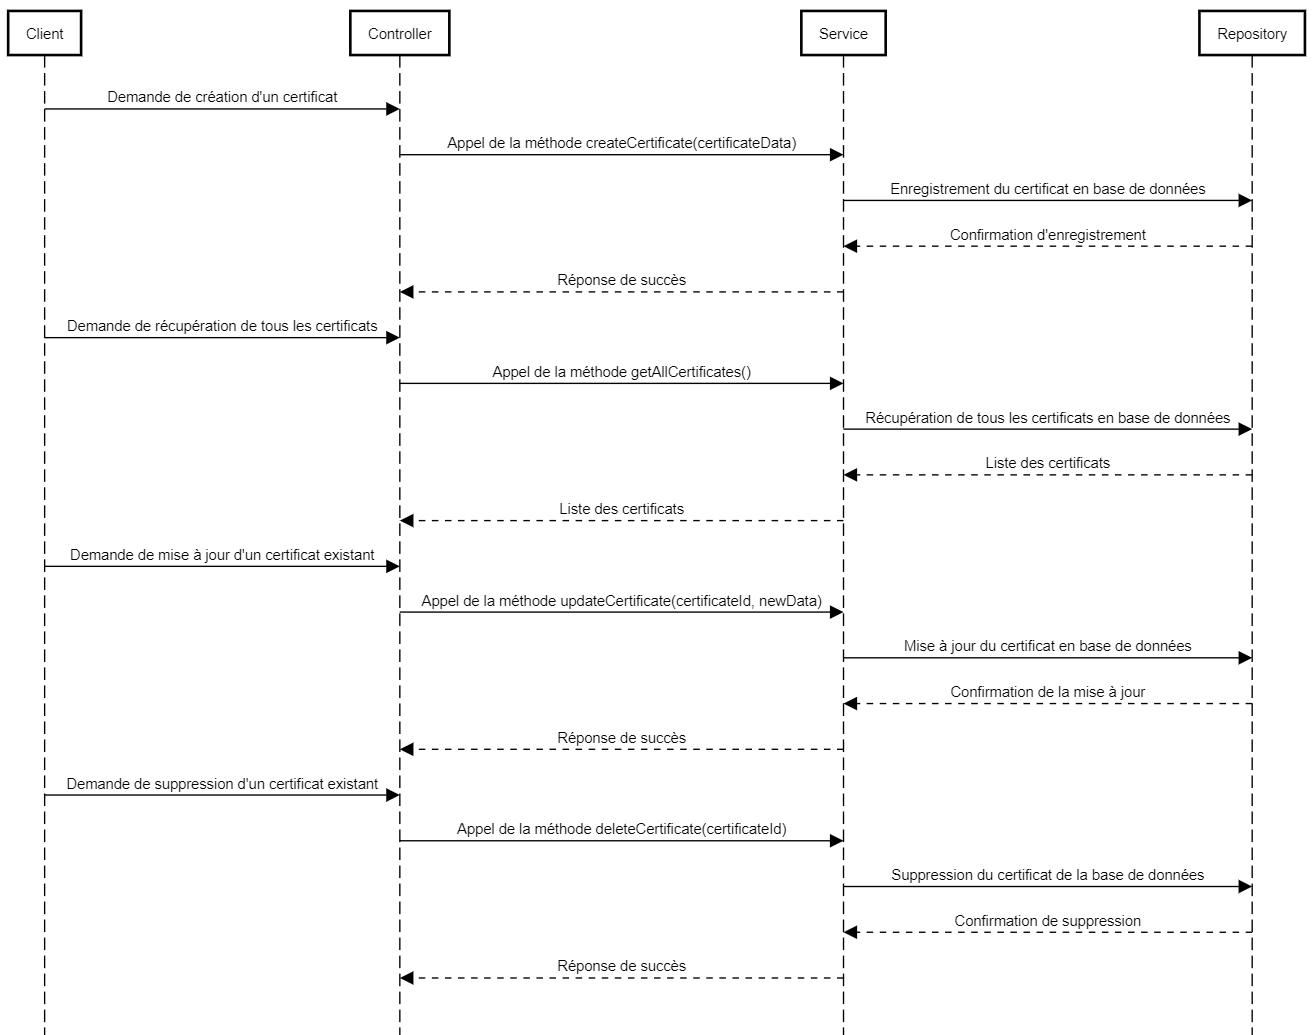
\includegraphics[width=\textwidth]{seq-certifs.png} 
\caption{Diagramme de sequence des certificats}
\label{fig:seq_certifs}
\end{figure}

\section{Realisation}
\begin{figure}
\centering
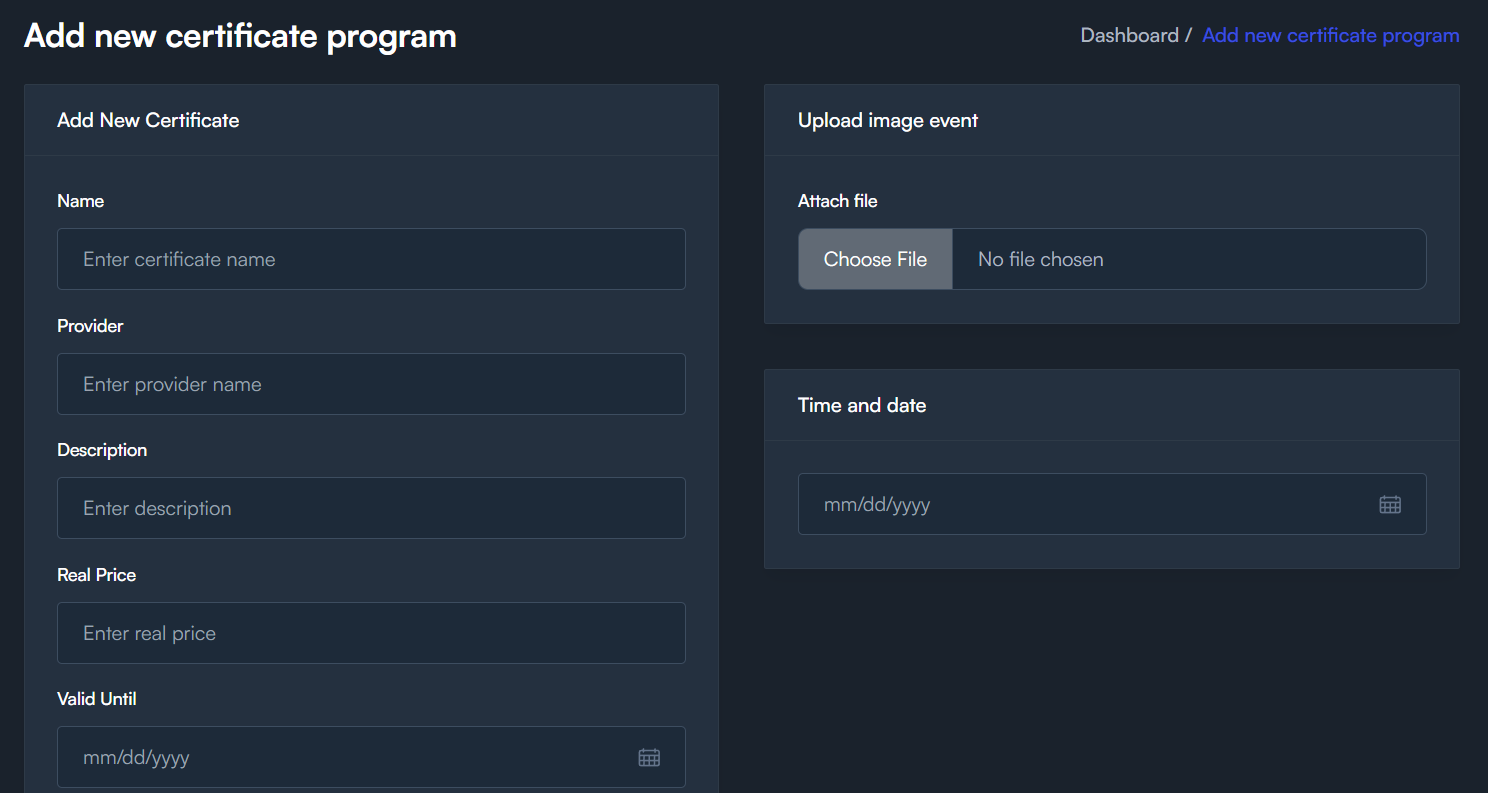
\includegraphics[width=\textwidth]{admin-add-certif.png} 
\caption{Ajout des certificats par le gestionnaire}
\label{fig:Ajout_des_certificats}
\end{figure}


\begin{figure}
\centering
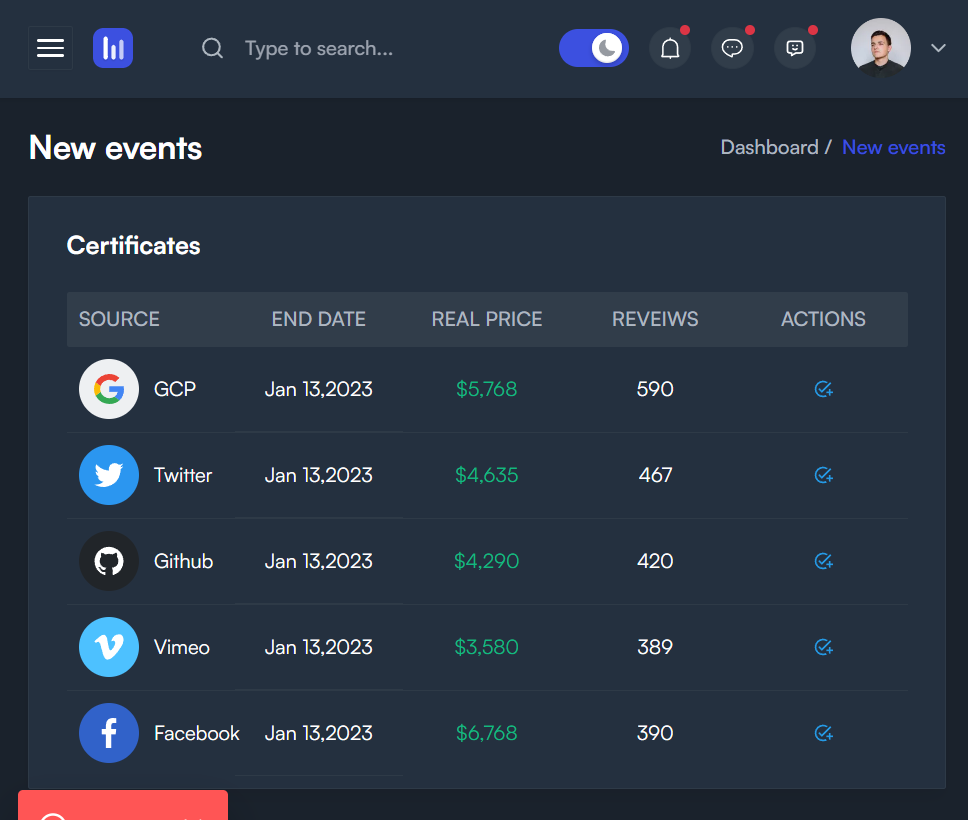
\includegraphics[width=\textwidth]{certifs-list.png} 
\caption{Liste des certificats disponibles}
\label{fig:certificates}
\end{figure}


\begin{figure}
\centering
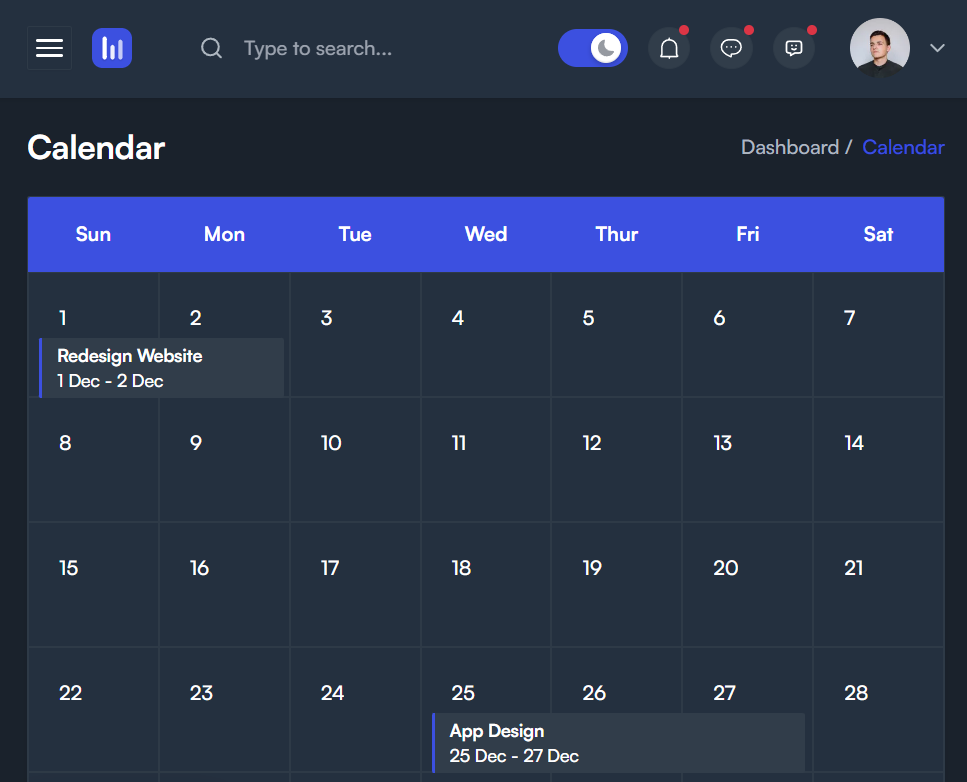
\includegraphics[width=\textwidth]{calendar.png} 
\caption{Le calendrier de l'etudiant avec les evenements auxquels il est inscrit}
\label{fig:calender}
\end{figure}



\clearpage

\chapter{MISE EN ŒUVRE DU SPRINT 4: Amelioration de lInterface Utilisateur et  deploiment et creation des contenaires}


\section{Introduction}
Le sprint 3 a ete consacre à l'amelioration de l'interface utilisateur (UI) et à l'optimisation des performances du chatbot, conformement aux User Stories 3.1 et 3.2. Cette phase a vise à ameliorer l'experience globale des utilisateurs et à garantir des performances optimales du chatbot. De plus, dans ce sprint, des conteneurs Docker ont ete crees pour chaque service, facilitant ainsi le deploiement et la gestion de l'ensemble du système. Voici les details de cette etape :


\section{Backlog du Sprint 4}

Le developpement de notre application de gestion de chatbot s’est structure autour d’un backlog produit bien defini, comprenant plusieurs epopees et user stories. Chaque user story a ete accompagnee de critères d’acceptation clairs pour garantir la qualite et la conformite aux attentes.

\subsection{epopee 2 : Developpement des Fonctionnalites de la Plateforme}

\textbf{User Story 2.2 : Inscription aux Cours et evenements}
\begin{itemize}
    \item \textbf{En tant que :} utilisateur
    \item \textbf{Je veux :} m'inscrire aux cours et evenements
    \item \textbf{Afin de :} participer à ceux-ci
    \item \textbf{Critères d'acceptation :}
    \begin{itemize}
        \item Les utilisateurs peuvent s'inscrire à des cours et des evenements via la plateforme.
        \item Un système de confirmation d'inscription est en place.
    \end{itemize}
\end{itemize}

\textbf{User Story 2.3 : Inscription aux Examens de Certification Gratuits}
\begin{itemize}
    \item \textbf{En tant que :} utilisateur
    \item \textbf{Je veux :} m'inscrire à des examens de certification gratuits
    \item \textbf{Afin de :} obtenir des certifications
    \item \textbf{Critères d'acceptation :}
    \begin{itemize}
        \item Les utilisateurs peuvent voir les examens de certification disponibles et s'y inscrire gratuitement.
        \item Un système de confirmation d'inscription aux examens est en place.
    \end{itemize}
\end{itemize}


\section{Analyse et Conception}
\subsection{Description textuel}
\begin{itemize}
    \item **Optimisation des Performances du Chatbot :** L'equipe a effectue une serie d'optimisations pour ameliorer le temps de reponse du chatbot. Cela comprenait des ajustements dans l'architecture du modèle, l'optimisation des requêtes et l'amelioration globale de l'efficacite des processus de traitement du langage naturel.
    
    \item **Amelioration de l'Interface Utilisateur :** L'interface utilisateur du chatbot a ete revue et amelioree pour offrir une experience plus conviviale et esthetique. Des fonctionnalites telles que le mode sombre et le mode clair ont ete ajoutees pour permettre aux utilisateurs de choisir leur preference visuelle. De plus, des animations ont ete integrees pour rendre l'interface plus dynamique et engageante.
    
    \item **Creation des Conteneurs Docker :** Dans le cadre de la preparation au deploiement, des conteneurs Docker ont ete crees pour chaque service du système. Cela inclut le chatbot, le service web, la base de donnees et tout autre composant necessaire. Les conteneurs Docker offrent une methode standardisee et portable pour empaqueter, distribuer et executer des applications, simplifiant ainsi le processus de deploiement et de gestion.
    
    \item **Tests de Performance et de Convivialite :** Des tests approfondis ont ete effectues pour evaluer l'impact des ameliorations apportees à l'interface utilisateur et aux performances du chatbot. Cela comprenait des tests de charge pour evaluer la stabilite du système sous charge maximale, ainsi que des tests d'utilisabilite pour evaluer la facilite d'utilisation de l'interface par les utilisateurs finaux.
\end{itemize}

Le sprint 4 a permis d'apporter des ameliorations significatives à l'experience utilisateur et aux performances du chatbot, tout en preparant le système à un deploiement efficace à l'aide de conteneurs Docker.

\subsection{Screenshots}

\begin{figure}
\centering
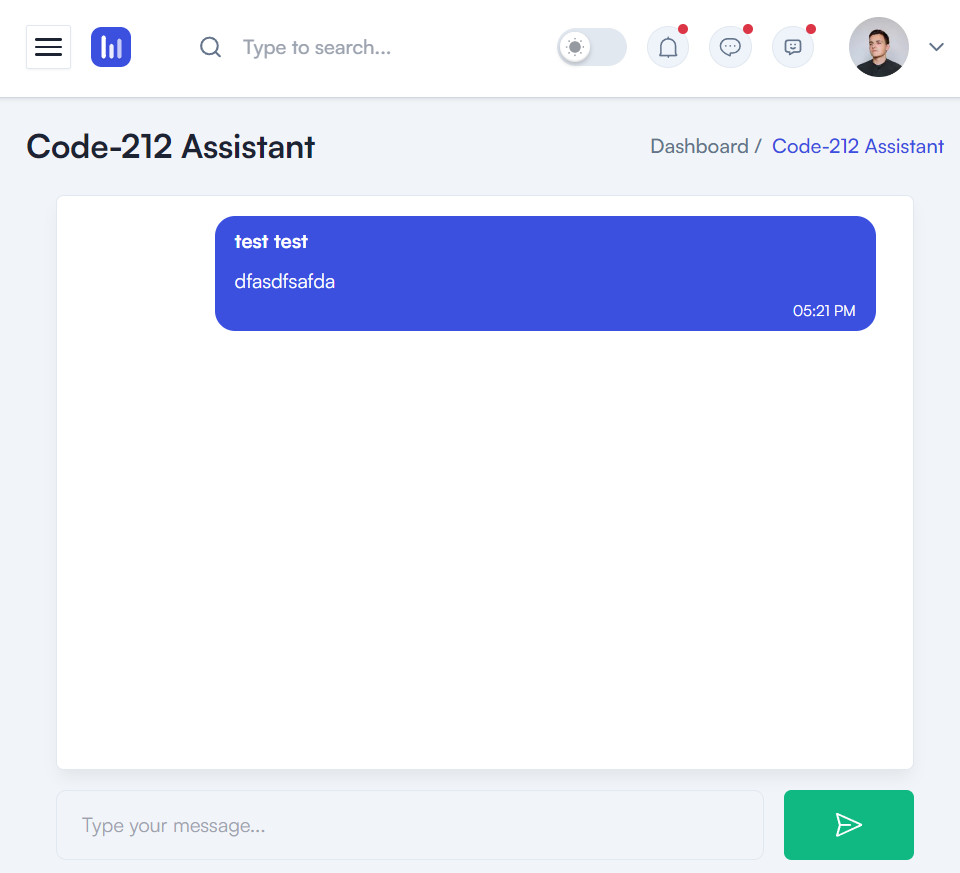
\includegraphics[width=\textwidth]{light-chat.png} 
\caption{Chat bot en light mode}
\label{fig:lightchat}
\end{figure}


\begin{figure}
\centering
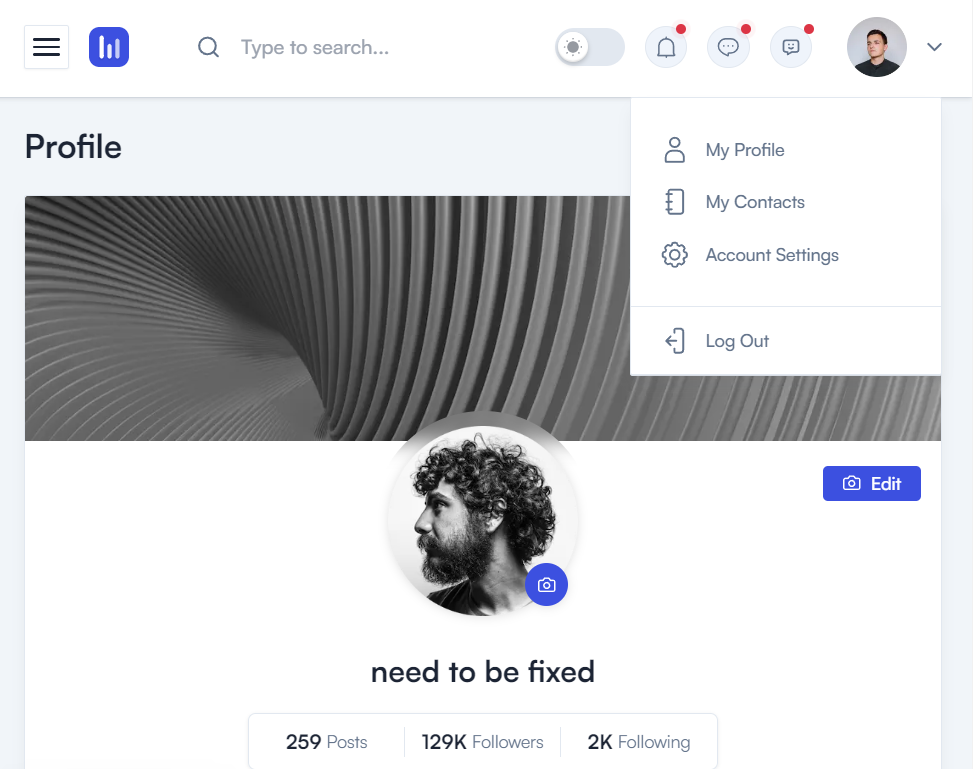
\includegraphics[width=\textwidth]{light-profile.png} 
\caption{Le profile d'utilisateur en light mode}
\label{fig:profile}
\end{figure}

\clearpage


\section{Deploiement et Infrastructure}
Le deploiement des microservices a ete realise à l'aide de conteneurs Docker, assurant une portabilite et une isolation des services. Docker a ete choisi en raison de sa capacite à empaqueter les applications et leurs dependances de manière coherente, garantissant que les services fonctionnent de manière identique sur n'importe quel environnement. 

Un Docker Compose a ete cree pour orchestrer les differents services et simplifier le deploiement de l'ensemble de l'application. Cette approche permet de definir et de gerer les services, les reseaux et les volumes dans un fichier YAML unique, facilitant ainsi le deploiement et la mise à l'echelle des microservices.

Kubernetes a ete utilise pour l'orchestration des conteneurs, permettant une gestion automatisee du deploiement, de la mise à l'echelle et de la maintenance des applications conteneurisees. Kubernetes a ete choisi pour sa robustesse, sa capacite à gerer des deploiements complexes et son large ecosystème de support. Il permet egalement de s'assurer que les applications sont hautement disponibles et peuvent se redimensionner en fonction des besoins.

\subsection{Environnement de Production}
L'environnement de production a ete configure pour garantir une haute disponibilite et une resilience face aux pannes. Des pratiques de surveillance et de logging ont ete mises en place pour assurer une surveillance proactive et une resolution rapide des incidents. Kubernetes facilite egalement la mise en place d'un environnement de production resilient grâce à ses capacites de gestion des defaillances et de repartition de charge.

\subsection{Securite}
Des mesures de securite ont ete integrees dès le debut du developpement, incluant l'utilisation de Keycloak pour la gestion des accès, la mise en place de pare-feu, et l'utilisation de certificats SSL pour les communications securisees. L'utilisation de Kubernetes ajoute une couche supplementaire de securite grâce à ses fonctionnalites natives, telles que la gestion des secrets et la definition de politiques de securite au niveau du cluster.



\section{Conclusion}
La realisation et la mise en œuvre de l'application ont suivi une approche structuree et methodique, garantissant le respect des delais et des exigences de qualite. L'utilisation de la methodologie agile, combinee à des technologies modernes et des pratiques de deploiement robustes, a permis de developper une application modulaire, scalable et securisee, repondant aux besoins des utilisateurs finaux.


\chapter{Conclusion Generale}

Ce rapport resume notre travail durant notre stage de fin d’annee au sein du centre Code212. Nous avons commence par introduire le contexte general du projet et les differents besoins et exigences, puis nous avons prepare un planning de travail en respectant les priorites des besoins. Nous avons consacre la partie suivante à l’etude technique et aux choix des outils et technologies. Ensuite, nous avons entame la realisation de chaque sprint.
\newline
Ce projet a eu pour objectif principal de developper et implementer un chatbot dote d'intelligence artificielle au sein de la plateforme e-learning de Code212. Cette initiative s'inscrit dans le contexte d'une digitalisation croissante de l'education, necessitant des outils innovants et reactifs pour repondre efficacement aux besoins des etudiants. Code212, en tant qu'acteur cle dans la formation numerique au Maroc, vise par cette demarche à ameliorer l'interaction et l'assistance offertes à ses apprenants, tout en optimisant ses ressources pedagogiques.
\newline

L'introduction du chatbot IA apporte des benefices multiples. Les etudiants beneficient d'une assistance instantanee pour leurs questions frequentes, ce qui facilite un apprentissage autonome et renforce le processus educatif. En fournissant des outils pratiques et interactifs pour la formation, Code212 prepare mieux ses etudiants à integrer le marche du travail numerique. De plus, le chatbot aide à une utilisation plus efficace des ressources pedagogiques disponibles, maximisant ainsi l'efficacite des etudes des apprenants. En offrant un soutien empathique et motivant, le chatbot contribue à maintenir la perseverance et l'engagement des etudiants.

Cependant, le projet n'a pas ete exempt de defis. La conception d'un système AI convivial a ete surmontee par une comprehension precise des besoins des utilisateurs et par des iterations continues basees sur les feedbacks. L'integration des technologies de pointe a ete geree efficacement grâce à une planification rigoureuse et à l'adoption de methodologies Agiles.
\newline

Le succès initial du chatbot IA ouvre de nouvelles perspectives pour Code212. Parmi les pistes de developpement futur, on envisage l'elargissement des fonctionnalites en ajoutant des capacites plus avancees comme l'analyse predictive pour anticiper les besoins des etudiants et offrir des suggestions proactives. Il est aussi envisage d'integrer le chatbot à d'autres systèmes educatifs, connectant ainsi des plateformes d'apprentissage en ligne et des outils de gestion academiques pour une experience d'apprentissage encore plus fluide. L'amelioration continue basee sur les retours des utilisateurs et les developpements technologiques sera essentielle pour rester à la pointe de l'innovation educative. L'optimisation du chatbot, en recherchant des methodes pour ameliorer les performances, y compris l'optimisation des algorithmes et l'utilisation de technologies de pointe pour reduire les temps de reponse, est egalement cruciale. Enfin, la mise en œuvre de techniques d'equilibrage de charge pour assurer une repartition efficace des demandes sur les serveurs garantira la disponibilite et la reactivite du chatbot même en periode de forte affluence.
\newline

En conclusion, l'integration d'un chatbot IA au sein de Code212 represente une avancee significative dans l'effort continu de modernisation et d'optimisation de l'education numerique au Maroc. Cette initiative repond non seulement aux besoins immediats des etudiants mais pose egalement les jalons pour un avenir où l'apprentissage est resolument aligne avec les opportunites et defis du monde numerique. Ainsi, Code212 confirme sa mission de former des professionnels qualifies et prêts à relever les defis de l'economie numerique, tout en renforçant son rôle de leader dans la transformation digitale de l'enseignement au Maroc.



\chapter*{Bibliographies et Webographie}

\begin{itemize}
    \item[1.] Jeff Sutherland and Ken Schwaber, "Scrum: A Comprehensive Guide to Agile Project Management", 3rd Edition, 2022.
    \item[2.] Guide de demarrage Scrum | L'Agiliste.
    \item[3.] \url{https://www.redhat.com/en/topics/integration/whats-the-difference-between-soaprest}
    \item[4.] \url{https://www.researchgate.net/figure/Client-server-architecture-and-technologies_fig1_353325675}
    \item[5.] \url{https://medium.com/@mindfiresolutions.usa/advantages-and-disadvantages-of-php-frameworks-c046d50754e5}
    \item[6.] \url{https://www.javatpoint.com/advantages-and-disadvantages-of-java}
    \item[7.] \url{https://en.wikipedia.org/wiki/Python_(programming_language)}
    \item[8.] \url{https://www.agilites.com/pros-and-cons-of-using-c-as-your-backend-programming-language.html}
    \item[9.] \url{https://medium.com/@mindfiresolutions.usa/advantages-and-disadvantages-of-php-frameworks-c046d50754e5}
    \item[10.] \url{https://www.javatpoint.com/advantages-and-disadvantages-of-java}
    \item[11.] \url{https://python.plainenglish.io/the-pros-and-cons-of-using-python-for-web-development-9134f2c4f16f}
    \item[12.] \url{https://en.wikipedia.org/wiki/Apache_Maven}
    \item[13.] \url{https://en.wikipedia.org/wiki/Apache_Ant}
    \item[14.] \url{https://en.wikipedia.org/wiki/Gradle}
    \item[15.] Laurentiu Spilca, "Spring Security in Action".
    \item[16.] Kim Hamilton and Russ Miles, "Learning UML 2.0".
    \item[17.] \url{https://www.amigoscode.com/p/spring-boot-security}
    \item[18.] \url{https://en.wikipedia.org/wiki/Spring_Framework}
    \item[19.] \url{https://en.wikipedia.org/wiki/Spring_FrameworkSpring_Boot}
    \item[20.] \url{https://en.wikipedia.org/wiki/Spring_Security}
    \item[21.] \url{https://www.infoq.com/articles/spring-data-intro/}
    \item[22.] \url{https://en.wikibooks.org/wiki/Java_Persistence/What_is_JPA%3F}
    \item[23.] \url{https://www.javatpoint.com/hibernate-tutorial}
    \item[24.] \url{https://fr.wikipedia.org/wiki/IntelliJ_IDEA}
    \item[25.] \url{https://www.blazemeter.com/blog/how-use-postman-manage-and-execute-your-apis}
    \item[26.] \url{https://en.wikipedia.org/wiki/Swagger_(software)}
    \item[27.] Craig Walls, "Spring in Action, Fifth Edition".
    \item[28.] \url{https://blog.logrocket.com/tailwind-css-is-it-tomorrows-bootstrap-ebe560f9d00b/}
    \item[29.] \url{https://fr.wikipedia.org/wiki/Bootstrap_(framework)}
    \item[30.] \url{https://en.wikipedia.org/wiki/HTML}
    \item[31.] \url{https://en.wikipedia.org/wiki/CSS}
    \item[32.] \url{https://en.wikipedia.org/wiki/JavaScript}
    \item[33.] \url{https://dev.to/cesareferrari/working-with-axios-in-react-540c}
    \item[34.] \url{https://en.wikipedia.org/wiki/JSON}
    \item[35.] \url{https://www.journaldev.com/10660/json-server}
    \item[36.] \url{https://en.wikipedia.org/wiki/Git}
    \item[37.] \url{https://en.wikipedia.org/wiki/GitHub}
    \item[38.] \url{https://en.wikipedia.org/wiki/GanttProject}
    \item[39.] \url{https://en.wikipedia.org/wiki/MySQL}
    \item[40.] \url{https://en.wikipedia.org/wiki/PostgreSQL}
    \item[41.] \url{https://huggingface.co/} - Hugging Face, plateforme pour les modèles de langage et les outils NLP.
    \item[42.] \url{https://langchain.com/} - LangChain, une bibliothèque pour la creation d'applications alimentees par des modèles de langage.
    \item[43.] \url{https://github.com/facebookresearch/llama} - LLaMA 2, un modèle de langage de Facebook AI Research.
    \item[44.] \url{https://fastapi.tiangolo.com/} - FastAPI, un framework web pour Python pour la construction d'API rapides et performantes.
\end{itemize}


\end{document}




